%!TeX root=../carlo_master.tex
\chapter{Experimental analysis: multiclass classification}\label{sec:multiclass_experiments}

This chapter evaluates the partition-optimization and Voronoi decision strategies of Chapters~\ref{sec:partition_optimization} and~\ref{sec:voronoi_tessellation} on eleven datasets, ten base classifiers, and twelve objectives (seven cost-sensitive objectives and five maximization metrics). The protocol adapts the binary setup of Chapter~\ref{sec:binary_experiments}, changing only the dataset pool, decision-strategy families, and objective set. The cross-validated tuning variants lead both objective groups. On cost objectives the top is shared by three variants within sampling noise (FullMatrixPartitioningCV, RiskPartitioningCV, LinearScalingCV, all between $78$ and $80\%$); on maximization metrics ThresholdRatioCV leads at $90\%$.

\section{Experimental setup}\label{sec:multiclass_setup}

We adapt the binary protocol of Section~\ref{sec:binary_experiments} to the multiclass case, changing the dataset pool, decision-strategy families, and objective set while keeping the data partition, preprocessing, and evaluation method identical.

\subsection{Datasets}
The benchmark draws eleven multiclass datasets from OpenML \citep{vanschoren2014openml}, selected along the same axes as the binary pool of Section~\ref{sec:binary_experiments} with imbalance diversity replaced by class-count spread: $K$ ranges from $3$ to $10$, exercising the partition-optimization strategies of Section~\ref{sec:partition_optimization} across simplex dimensions where the number of decision-boundary parameters grows with the number of classes. Sample sizes span $N=150$ to $N\approx 83\text{k}$ across the same three tiers, and the pool recovers the core multiclass datasets of \citet{obrien2008costsensitive}, extended with larger-$N$ and higher-$K$ tasks.

Table~\ref{tab:dataset-summary-multiclass} summarizes the datasets. Preprocessing follows the binary pipeline (Section~\ref{sec:binary_experiments}): median imputation and standardization for numerical features, most-frequent imputation and one-hot encoding for categorical features, fitted once per dataset prior to splitting.

\begin{table}[H]
  \centering
  \caption{Summary of multiclass classification datasets used in the experiments. Superscripts denote OpenML dataset IDs. Numerical and Categorical are the counts of raw numerical and categorical input features; Encoded is the model input dimensionality after one-hot encoding of the categorical features. The imbalance ratio (IR) is the size of the majority class divided by that of the minority class.}%
  \label{tab:dataset-summary-multiclass}
  \resizebox{\textwidth}{!}{%
  \begin{tabular}{lrrrrrl}
\toprule
 &  &  & \multicolumn{3}{c}{Features} &  \\
\cmidrule(lr){4-6}
Dataset & Samples & Classes & Numerical & Categorical & Encoded & IR \\
\midrule
iris\textsuperscript{\tiny 61}~\citep{fisher1936iris} & 150 & 3 & 4 & 0 & 4 & 1.0 \\
vehicle\textsuperscript{\tiny 54}~\citep{siebert1987vehicle} & 846 & 4 & 18 & 0 & 18 & 1.1 \\
cmc\textsuperscript{\tiny 23}~\citep{lim2000cmc} & 1473 & 3 & 2 & 7 & 24 & 1.9 \\
yeast\textsuperscript{\tiny 181}~\citep{horton1996yeast} & 1484 & 10 & 8 & 0 & 8 & 92.6 \\
wine\_quality\_red\textsuperscript{\tiny 40691}~\citep{cortez2009wine} & 1599 & 6 & 11 & 0 & 11 & 68.1 \\
abalone\textsuperscript{\tiny 1557}~\citep{nash1994abalone} & 4177 & 3 & 7 & 1 & 10 & 1.1 \\
fot\_proving\textsuperscript{\tiny 1475}~\citep{bridge2014fol} & 6118 & 6 & 51 & 0 & 51 & 5.3 \\
satimage\textsuperscript{\tiny 182}~\citep{srinivasan1993satimage} & 6430 & 6 & 36 & 0 & 36 & 2.4 \\
gesture\_phase\textsuperscript{\tiny 4538}~\citep{madeo2013gesture} & 9873 & 5 & 32 & 0 & 32 & 3.0 \\
volkert\textsuperscript{\tiny 41166}~\citep{guyon2015automl} & 58310 & 10 & 180 & 0 & 180 & 9.4 \\
jannis\textsuperscript{\tiny 41168}~\citep{guyon2015automl} & 83733 & 4 & 54 & 0 & 54 & 22.8 \\
\bottomrule
\end{tabular}
  }
\end{table}


\subsection{Estimator architectures}
The ten base classifiers from the binary setup (Section~\ref{sec:binary_experiments}) carry over unchanged. Following the usage guidelines of TabPFN \citep{hollmann2025accurate} and TabICL \citep{qu2025tabicl} (labeled TabICL in the result tables), which cap the training set at roughly ten thousand samples, both are skipped on the two largest datasets (\textit{volkert}, \textit{jannis}), and TabICL is additionally skipped on the smallest (\textit{iris}) by its documented input gates, leaving those (dataset, model) cells absent from the results.

\subsection{Objectives}\label{sec:multiclass_objectives}
The objective set covers twelve targets: five maximization metrics (macro $F_1$, macro $F_2$, macro $F_{0.5}$, MCC, and macro G-Mean) and seven cost-sensitive objectives (six $K$-parameterized cost matrices and Balanced Accuracy in its prior-weighted cost-matrix form, see Section~\ref{sec:binary_objectives}).

The four \emph{macro} metrics share the same one-vs-rest reduction: for each class $k \in \mathcal{Y}$, examples with true label $k$ are treated as positives and all others as negatives, yielding per-class counts $\mathrm{TP}_k$, $\mathrm{FP}_k$, $\mathrm{FN}_k$ from the $K \times K$ test confusion matrix. The macro aggregate combines the $K$ per-class scores with equal weight across classes (independent of the class priors). For $F_\beta$ that aggregate is the arithmetic mean of per-class $F_\beta$ scores,
\begin{equation*}
F_\beta^{\mathrm{macro}} = \frac{1}{K}\sum_{k=1}^{K} \frac{(1+\beta^2)\,\mathrm{TP}_k}{(1+\beta^2)\,\mathrm{TP}_k + \beta^2\,\mathrm{FN}_k + \mathrm{FP}_k},
\end{equation*}
implemented as \texttt{sklearn.\allowbreak metrics.\allowbreak fbeta\_\allowbreak score(average=`macro')}. For G-Mean the per-class score is the true-positive rate $\mathrm{TPR}_k = \mathrm{TP}_k / (\mathrm{TP}_k + \mathrm{FN}_k)$ and the aggregate is the geometric mean,
\begin{equation*}
\mathrm{GMean}^{\mathrm{macro}} = \Big(\prod_{k=1}^{K} \mathrm{TPR}_k\Big)^{\!1/K},
\end{equation*}
implemented as \texttt{imblearn.\allowbreak metrics.\allowbreak geometric\_\allowbreak mean\_\allowbreak score(average=`macro')}. MCC is not a per-class score and so does not use this reduction; it generalises to $K > 2$ as a single scalar computed directly from the full $K \times K$ confusion matrix in the \citet{gorodkin2004comparing} formulation (\texttt{sklearn.\allowbreak metrics.\allowbreak matthews\_\allowbreak corrcoef}). These five maximization metrics are non-decomposable in the sense of \citet{narasimhan2015optimizing}, as discussed in Section~\ref{sec:binary_objectives}.

The cost-sensitive objectives are:
\begin{itemize}
    \item Symmetric: $0/1$ loss ($C_{ij} = 0$ if $i = j$, else $1$).
    \item Asymmetric $10\times$ / Asymmetric $100\times$: unit costs with a $10\times$ or $100\times$ penalty on errors involving the last class.
    \item Custom: A hand-specified matrix for $K\!=\!3$ ($C_{12} = C_{21} = 5$, other off-diagonals $1$).
    \item Ordinal: $C_{ij} = |i - j|$.
    \item Quadratic: $C_{ij} = (i - j)^2$ \citep{obrien2008costsensitive}.
    \item Balanced Error: the prior-weighted form of Section~\ref{sec:binary_objectives}, generalized to $K > 2$ as $1 - \texttt{sklearn.\allowbreak metrics.\allowbreak balanced\_\allowbreak accuracy\_\allowbreak score}$ (one minus the unweighted mean of per-class recalls, equivalent to misclassification weights $1/(K\pi_y)$ on class $y$ under per-sample-average risk).
\end{itemize}
The two distance-based matrices model class labels with an implicit ordering, such as severity grades or quality tiers, where confusing adjacent classes is less costly than confusing distant ones.

\subsection{Decision strategies}\label{sec:multiclass_strategies}
For each combination of dataset, model, and objective we evaluate twenty-four strategies mapping a probability vector $\hat{\mathbf{p}}(x) \in \Delta^{K-1}$ to a class label. Each tuning strategy is one of the parameterizations of the partition-matrix framework analyzed in Section~\ref{sec:partition_optimization}: the baselines fix $\mathbf{A} = \mathbf{C}$ (the analytical rule of Eq.~\ref{eq:multiclass_bayes}) or ignore the cost matrix, the vector-tuned and full-matrix families learn $\mathbf{A}$ under the structural constraints of Section~\ref{sec:partition_matrix_framework}, and the Voronoi family replaces the linear partition with a nearest-prototype tessellation (Section~\ref{sec:voronoi_tessellation}). They are presented in order of increasing hypothesis-class complexity (the $\mathcal{H}_{PS}$, $\mathcal{H}_{Vor}$, $\mathcal{H}_{Full}$ hierarchy of Table~\ref{tab:partition_natarajan}), with the priority-based cascade of Section~\ref{sec:sequential_selection} grouped on its own since its non-convex, order-dependent regions fall outside that hierarchy. Following Section~\ref{sec:partition_optimization}, we refer to $\mathcal{H}_{PS} \cup \mathcal{H}_{Sc} \cup \mathcal{H}_{Full}$ collectively as the \emph{matrix-parameterized methods} and to the $K-1$-parameter subset $\mathcal{H}_{PS} \cup \mathcal{H}_{Sc}$ as the \emph{vector-tuned methods}.

\paragraph{Uncalibrated and calibrate-then-decide baselines.}
\begin{itemize}
    \item Argmax: The cost-blind rule $\mathrm{argmax}_{k \in \mathcal{Y}} \hat{p}_k$.
    \item Analytical: The Bayes-optimal projection $\mathrm{argmin}_{k \in \mathcal{Y}} \mathbf{c}_k^\top \hat{\mathbf{p}}$ (Eq.~\ref{eq:multiclass_bayes}) applied to uncalibrated scores; the fixed point $\mathbf{A} = \mathbf{C}$ of the partition-matrix framework that every tuning strategy below departs from.
    \item {\sloppy IsotonicArgmax, PlattScalingArgmax, TemperatureScalingArgmax, DirichletCalibrationArgmax: Post-hoc calibration (isotonic one-vs-rest, Platt one-vs-rest, single-parameter temperature, and Dirichlet; Section~\ref{sec:multiclass_calibration}) followed by $\mathrm{argmax}$.\par}
    \item {\sloppy IsotonicAnalytical, PlattScalingAnalytical, TemperatureScalingAnalytical, DirichletCalibrationAnalytical: The same four calibrators (Section~\ref{sec:multiclass_calibration}) followed by the analytical rule of Eq.~\ref{eq:multiclass_bayes} instead of $\mathrm{argmax}$.\par}
\end{itemize}

\paragraph{Vector-tuned partition methods.} These strategies are the vector-parameterized members of the partition-matrix framework (Section~\ref{sec:partition_optimization}). Each learns a single $K$-vector that translates or rescales the polyhedral boundaries of the standard partition, keeping the decision rule within the vector-tuned subset $\mathcal{H}_{PS} \cup \mathcal{H}_{Sc}$ (per-class bias gives $\mathcal{H}_{PS}$ with $d_{Nat} = K-1$; per-class scaling gives $\mathcal{H}_{Sc}$ with $d_{Nat} \leq K-1$):
\begin{itemize}
    \item ThresholdRatio: Probability ratio thresholding (Section~\ref{sec:prob_ratio_thresholding}, Eq.~\ref{eq:threshold_ratio}). Per-class scalar rescaling $\hat{p}_k / \tau_k$ prior to $\mathrm{argmax}$, with the per-class ratios $\tau_k$ sampled by random search from $[0.01,\, 1.5]$. The range is asymmetric because $\tau_k \to 0$ amplifies $\hat{p}_k/\tau_k$ unboundedly while $\tau_k > 1.5$ would suppress class $k$ to the point of never being selected against competitors with $\tau_j$ near $1$.
    \item MultidimensionalThreshold: The simplex-side parameterization of \citet{marchetti2025multidimensional} (Section~\ref{sec:multidim_thresholding}), a per-class additive bias $\hat{p}_k - b_k$ prior to $\mathrm{argmax}$, with the per-class biases $b_k$ sampled by random search from $[-1, 1]$ (one class pinned at $b_k = 0$ for identifiability, so $K-1$ free parameters) and warm-started at $\mathbf{b} = \mathbf{0}$, so that Argmax is a fixed point; equivalent to the parallel-shift rule under $0/1$ loss (Proposition~\ref{prop:marchetti_equivalence}).
    \item RiskPartitioning: O'Brien's parallel-shift regularization (Section~\ref{sec:parallel_shifts}), the affine bias $A_{ij} = C_{ij} + \alpha_j$ on the cost matrix, fit by the changepoint solver of \citet{obrien2008costsensitive}. By Proposition~\ref{prop:parallel_invariance} it translates the cost-induced boundaries along the fixed normals $\mathbf{c}_i - \mathbf{c}_j$ without rotating them.
    \item LinearScaling: O'Brien's linear class scaling (Section~\ref{sec:linear_scaling}), the row-wise rescaling $A_{ij} = C_{ij}\beta_i$ of the cost matrix, equivalently the per-class probability reweighting of \citet{lachiche2003improving}. The per-truth-class weights $\boldsymbol{\beta} \in \mathbb{R}^K_{\ge 0}$ are sampled by random search from $[0,\, 5]$ and warm-started at $\boldsymbol{\beta} = \mathbf{1}$, so that Analytical is a fixed point; the lower bound of $0$ enforces $\beta_k \ge 0$ (a negative weight would invert the sign of truth class $k$'s costs), and only the ratios $\beta_i/\beta_j$ affect the prediction. By Proposition~\ref{prop:column_rotation} it rotates the cost-induced boundaries instead of translating them, the cost-aware counterpart of ThresholdRatio (the two coincide under $0/1$ loss with $\beta_k = 1/\tau_k$, Proposition~\ref{prop:ratio_equivalence}).
\end{itemize}

\paragraph{Priority-based cascade.} SequentialSelection is the threshold cascade of Section~\ref{sec:sequential_selection} (Eq.~\ref{eq:sequential_selection}), with $K{-}1$ scalar thresholds sampled by random search from $[0, 1]$ and applied in ascending-count (minority-first) order, so the rarest training class is the first candidate at every prediction. Its first-match-with-default structure yields non-convex, order-dependent decision regions, so it sits outside the $\mathcal{H}_{PS}/\mathcal{H}_{Vor}/\mathcal{H}_{Full}$ hierarchy at a parameter budget comparable to the vector-tuned methods.

\paragraph{Voronoi partition tuning.} The Voronoi hypothesis class $\mathcal{H}_{Vor}$ (Section~\ref{sec:voronoi_tessellation}) replaces the linear partition with a nearest-prototype tessellation of $\Delta^{K-1}$, allowing boundaries to rotate as well as translate at a parameter count of $K(K-1)$ for the simplex-restricted class and a Natarajan-dimension bound $d_{Nat} \le K^2$ (the middle tier of Table~\ref{tab:partition_natarajan}). VoronoiTuning performs a random search over prototype configurations drawn from Sequential $d^2$ (Algorithm~\ref{alg:voronoi_tuning}), which satisfies the Dominant Label Constraint (Definition~\ref{def:dlc}) by construction.

\paragraph{Full-matrix partition tuning.} The unconstrained partition class $\mathcal{H}_{Full}$ (Section~\ref{sec:partition_optimization}) learns all $K^2$ entries of the partition matrix $\mathbf{A}$ in the apparent-risk rule of Eq.~\ref{eq:obrien_rule}, $\delta_{\mathbf{A}}(\mathbf{p}) = \mathrm{argmin}_{i \in \mathcal{Y}} \mathbf{a}_i^\top \mathbf{p}$, the $d_{Nat} \le K^2$ ceiling of the framework. It is the parameterization \citet{obrien2008costsensitive} introduced before imposing the structural constraints that the parallel-shift family (Section~\ref{sec:parallel_shifts}) restricts to.

FullMatrixPartitioning parameterizes $\mathbf{A} = \mathbf{A}_0 + \boldsymbol{\Delta}$ around an anchor $\mathbf{A}_0$ and samples the perturbation $\boldsymbol{\Delta} \in [-1, 1]^{K \times K}$ by random search. The anchor is the cost matrix $\mathbf{C}$ for cost-sensitive objectives and the $0/1$ loss matrix $\mathbf{1}\mathbf{1}^\top - \mathbf{I}$ (off-diagonal entries $1$, diagonal entries $0$) for non-decomposable metrics, so that $\boldsymbol{\Delta} = \mathbf{0}$ reproduces Analytical or Argmax respectively.

The matrix analogue of the Dominant Label Constraint (Definition~\ref{def:dlc}), $A_{jj} \leq A_{ji}$ for all $i \neq j$, is not imposed, matching the unconstrained $\mathcal{H}_{Full}$ row of Table~\ref{tab:partition_natarajan}. Consequently the learned $\mathbf{A}$ need not be admissible (Definition~\ref{def:admissibility}) even when the evaluation matrix $\mathbf{C}$ is: an unconstrained $\mathbf{A}$ can leave some action $i$ dominated everywhere on $\Delta^{K-1}$, so that $\mathcal{P}_i^{\mathbf{A}} = \emptyset$ and class $i$ is never predicted. Keeping each vertex $\mathbf{e}_i$ in its own region, the property the Dominant Label Constraint enforces, is what rules out this empty-region case.

\paragraph{Cross-validated tuning variants.} For each tuning strategy above, we additionally evaluate a CV variant (ThresholdRatioCV, MultidimensionalThresholdCV, SequentialSelectionCV, RiskPartitioningCV, LinearScalingCV, VoronoiTuningCV, FullMatrixPartitioningCV) that selects parameters by 5-fold stratified cross-validation on the full train-full partition, eliminating the dedicated validation split. These variants use the same training data as Argmax and Analytical, which improves robustness on small datasets at the cost of a $5\times$ increase in fit time for the underlying base classifier.

\paragraph{Search budget.} Every tuning strategy that relies on stochastic search (ThresholdRatio, MultidimensionalThreshold, SequentialSelection, LinearScaling, VoronoiTuning, FullMatrixPartitioning, and their CV variants) uses random search with a fixed budget of $T = 301$ configurations per fit, drawn i.i.d.\ from the per-strategy ranges listed above ($\tau_k \in [0.01, 1.5]$, $b_k \in [-1, 1]$, SequentialSelection thresholds in $[0, 1]$, $\beta_k \in [0, 5]$, $\boldsymbol{\Delta} \in [-1, 1]^{K \times K}$). Each search is initialized at the analytical or $\arg\max$ fixed point of its parameterization ($\boldsymbol{\tau} = \mathbf{1}$, $\mathbf{b} = \mathbf{0}$, $\boldsymbol{\beta} = \mathbf{1}$, $\boldsymbol{\Delta} = \mathbf{0}$, or the standard argmax prototypes for VoronoiTuning) and the incumbent is replaced only on strict improvement of the validation objective (its cross-validated average for the CV variants), so each tuned strategy is no worse than its baseline on the tuning signal by construction. VoronoiTuning draws each of the $T$ configurations from the Sequential $d^2$ sampler (Algorithm~\ref{alg:voronoi_tuning}) with retry budget $M = 500$. RiskPartitioning is the exception: it is solved by the \citet{obrien2008costsensitive} changepoint algorithm rather than by sampling, and its CV variant reuses the same $T = 301$ random-search budget over the bias vector in $[-1, 1]^{K-1}$. A single random-search budget of $T = 301$ applies to every decision-layer search in this work. The binary campaign of Section~\ref{sec:binary_experiments} stands apart from this uniform setting: it optimizes its single threshold by exhaustive grid search ($G = 301$ points on $[0, 1]$) and so carries no sampling budget.

\subsection{Evaluation protocol}
The data partition matches the binary setup of Section~\ref{sec:binary_experiments}: $80\%$ train-full / $20\%$ test, with $70\%$ training / $10\%$ validation nested inside train-full.

Strategies consume different data budgets: Argmax and Analytical fit the base estimator on the full $80\%$ pool; calibration and hold-out tuning strategies fit on the $70\%$ training split and tune on the $10\%$ validation split; CV strategies cross-validate within the $80\%$ pool with the estimator fit anew on each fold.

The reported metric is the objective value on the held-out $20\%$ test set, averaged over $5$ independent seeds.

\section{Results and discussion}

Table~\ref{tab:model-auc-multiclass} reports the held-out test ROC AUC of each base estimator, computed one-vs-rest and weighted by class frequency, averaged over the ten seeds. The values fall within the ranges published for these datasets, so the comparison operates on estimators with the expected discriminative performance.

\begin{table}[H]
    \centering
    \footnotesize
    \caption{Held-out test ROC AUC of each base estimator trained on the full 80\% training pool (one-vs-rest, class-frequency-weighted) for the multiclass datasets, reported as mean $\pm$ 1 SE over the ten seeds. Models skipped by a documented sample-size, feature-count, or class-count gate have no entry. Bold marks every model within 1 SE of the per-dataset best.}%
    \label{tab:model-auc-multiclass}
    \adjustbox{max width=\linewidth}{%
    \begin{tabular}{lcccccccccc}
    \toprule
    Dataset & LGBM & LogReg & XGB & CatBoost & RF & ET & GaussNB & TabM & TabPFN & TabICL \\
    \midrule
    iris & 0.989 ± 0.005 & \textbf{0.998 ± 0.001} & 0.977 ± 0.007 & 0.996 ± 0.002 & \textbf{0.998 ± 0.001} & \textbf{0.998 ± 0.001} & 0.996 ± 0.001 & \textbf{0.998 ± 0.001} & \textbf{0.999 ± 0.001} & — \\
    vehicle & 0.932 ± 0.004 & 0.945 ± 0.003 & 0.929 ± 0.005 & 0.938 ± 0.004 & 0.932 ± 0.003 & 0.929 ± 0.004 & 0.771 ± 0.004 & 0.965 ± 0.003 & \textbf{0.979 ± 0.003} & \textbf{0.982 ± 0.002} \\
    cmc & 0.706 ± 0.008 & 0.687 ± 0.005 & 0.700 ± 0.007 & 0.705 ± 0.006 & 0.682 ± 0.005 & 0.632 ± 0.005 & 0.646 ± 0.006 & 0.713 ± 0.006 & \textbf{0.753 ± 0.006} & \textbf{0.753 ± 0.007} \\
    yeast & 0.821 ± 0.005 & 0.825 ± 0.004 & 0.826 ± 0.005 & 0.837 ± 0.006 & 0.844 ± 0.005 & 0.845 ± 0.006 & 0.728 ± 0.007 & 0.825 ± 0.005 & 0.847 ± 0.004 & \textbf{0.857 ± 0.005} \\
    wine\_quality\_red & 0.839 ± 0.005 & 0.758 ± 0.005 & 0.839 ± 0.005 & 0.840 ± 0.005 & 0.854 ± 0.005 & 0.867 ± 0.006 & 0.730 ± 0.006 & 0.796 ± 0.006 & 0.858 ± 0.005 & \textbf{0.878 ± 0.005} \\
    abalone & 0.825 ± 0.002 & 0.830 ± 0.002 & 0.824 ± 0.003 & 0.829 ± 0.002 & 0.825 ± 0.002 & 0.821 ± 0.002 & 0.774 ± 0.002 & 0.840 ± 0.002 & \textbf{0.851 ± 0.002} & \textbf{0.852 ± 0.002} \\
    fot\_proving & 0.868 ± 0.001 & 0.727 ± 0.001 & 0.867 ± 0.001 & 0.866 ± 0.002 & 0.866 ± 0.001 & 0.853 ± 0.001 & 0.628 ± 0.003 & 0.840 ± 0.002 & 0.877 ± 0.001 & \textbf{0.885 ± 0.001} \\
    satimage & 0.992 ± 0.000 & 0.981 ± 0.001 & 0.992 ± 0.000 & 0.993 ± 0.000 & 0.991 ± 0.000 & 0.992 ± 0.000 & 0.961 ± 0.001 & 0.993 ± 0.000 & 0.996 ± 0.000 & \textbf{0.996 ± 0.000} \\
    gesture\_phase & 0.888 ± 0.001 & 0.757 ± 0.001 & 0.892 ± 0.001 & 0.898 ± 0.001 & 0.890 ± 0.001 & 0.903 ± 0.001 & 0.718 ± 0.002 & 0.882 ± 0.001 & 0.948 ± 0.001 & \textbf{0.961 ± 0.001} \\
    volkert & 0.937 ± 0.000 & 0.888 ± 0.001 & 0.939 ± 0.000 & 0.941 ± 0.000 & 0.928 ± 0.000 & 0.928 ± 0.000 & 0.825 ± 0.001 & \textbf{0.952 ± 0.000} & — & — \\
    jannis & 0.872 ± 0.001 & 0.809 ± 0.001 & 0.873 ± 0.001 & 0.876 ± 0.001 & 0.862 ± 0.001 & 0.853 ± 0.001 & 0.739 ± 0.001 & \textbf{0.892 ± 0.001} & — & — \\
    \bottomrule
\end{tabular}
    }
\end{table}


The cross-validated tuning variants lead both objective groups. On cost objectives three CV variants are tied at the top within sampling noise: FullMatrixPartitioningCV ($80\%$ of cost cells won or tied), RiskPartitioningCV ($79\%$), and LinearScalingCV ($78\%$). On maximization metrics ThresholdRatioCV leads at $90\%$. The bare Analytical rule is the strongest non-tuning strategy on cost at $69\%$.

Per-dataset means $\pm\,1$ standard error (SE) over the ten seeds for every (model, objective, strategy) combination are reported in the companion supplement (\texttt{tex/supplement/supplement.pdf} in the source repository), in a cost-matrix table (all $24$ strategies) and a maximization-metric table, with the same bolding convention as the binary supplement. As in the binary chapter the within-$1$-SE rule is descriptive, not a per-cell significance test. The aggregates cover all ten base classifiers.

\subsection{Analytical thresholds under cost asymmetry}

Under the Symmetric matrix the analytical rule and the cost-blind Argmax coincide, since the cost-weighted argmin reduces to the argmax.

As the asymmetry grows the cost-blind rule degrades while the analytical rule, which folds the cost matrix into the decision, stays closer to the per-row best. Analytical wins or ties the per-row best on $69\%$ of cost cells, against $31\%$ for Argmax. The cross-validated tuning variants improve on this further, with the largest gains on the heavy-asymmetry matrices.

Figure~\ref{fig:ci-abalone-quadratic_cost} shows a representative cell, \textit{abalone} with LGBM under Quadratic: the cross-validated tuning variants, Analytical, and the parametric calibrate-then-analytical pipelines lead, the single-split tuning strategies follow, and the cost-blind strategies trail.

% Auto-generated by experiments.analysis.generate_ci_plots --- do not edit.
\begin{figure}[H]
\centering
\adjustbox{max width=\textwidth}{%
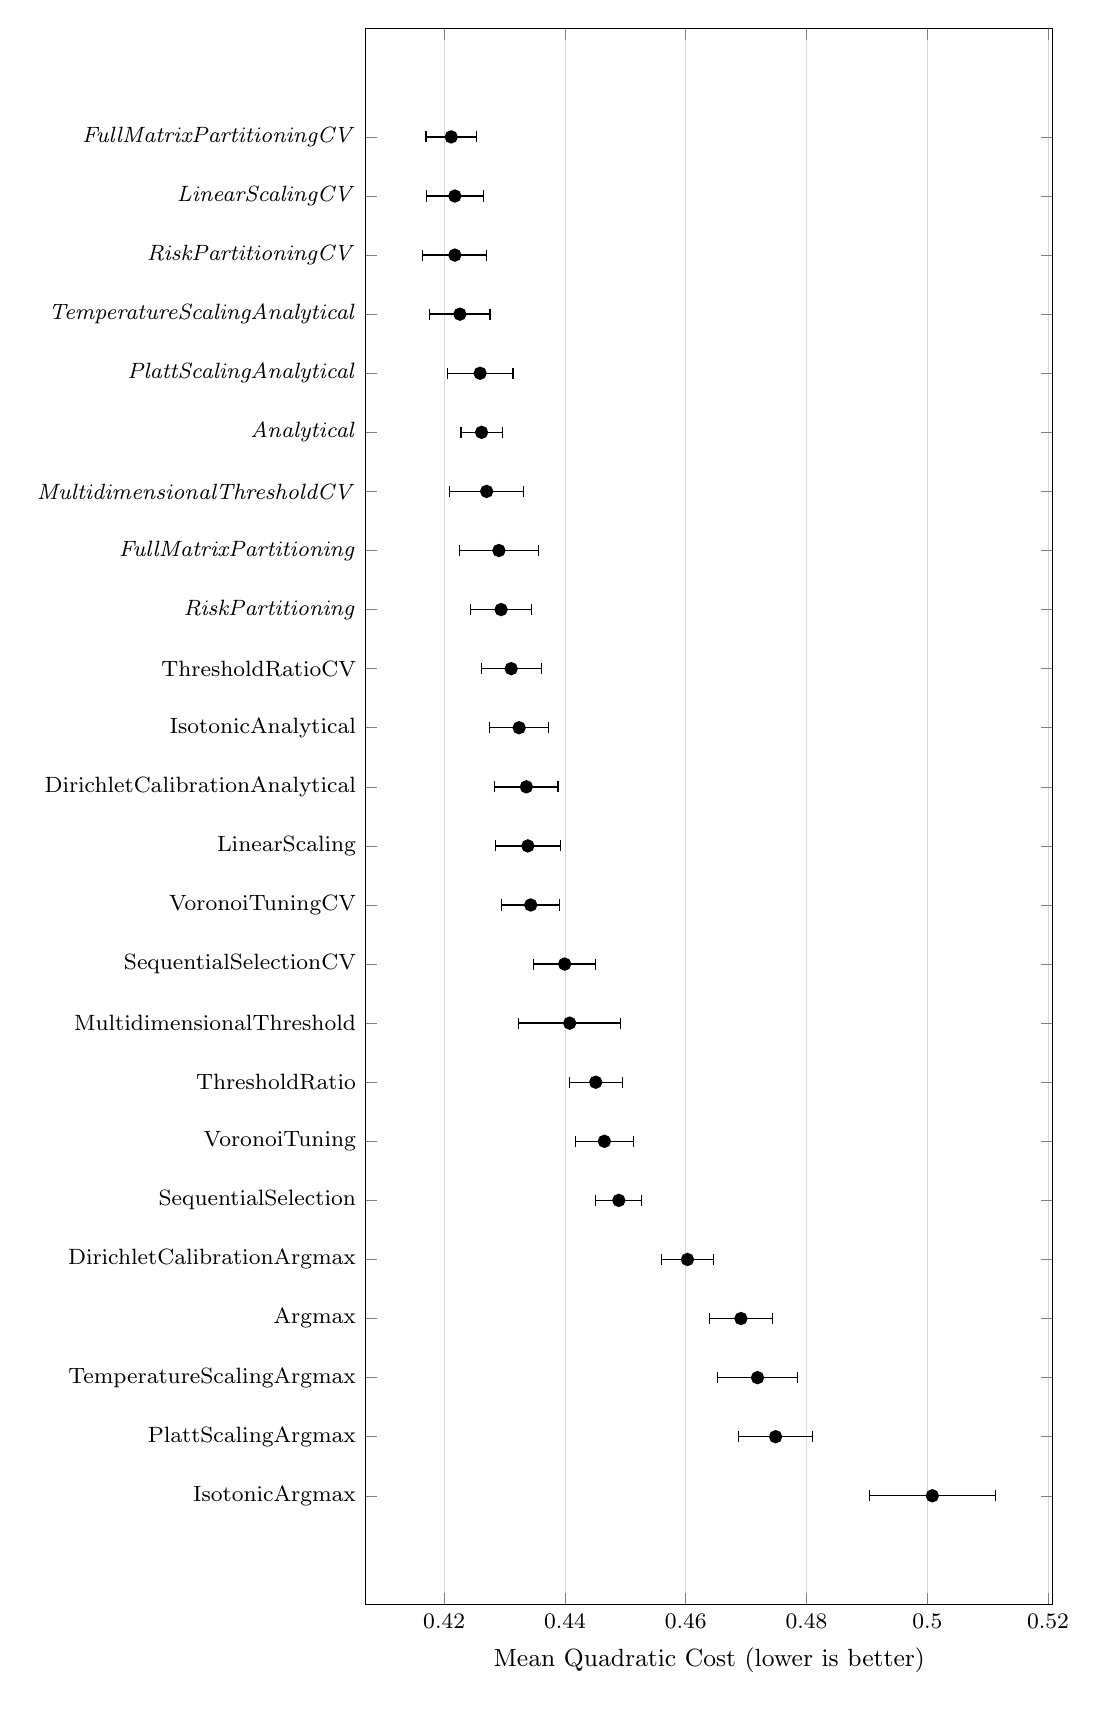
\begin{tikzpicture}
\begin{axis}[
    width=0.85\textwidth, height=21.60cm,
    xlabel={Mean Quadratic Cost (lower is better)},
    symbolic y coords={{FullMatrixPartitioningCV},{LinearScalingCV},{RiskPartitioningCV},{TemperatureScalingAnalytical},{PlattScalingAnalytical},{Analytical},{MultidimensionalThresholdCV},{FullMatrixPartitioning},{RiskPartitioning},{ThresholdRatioCV},{IsotonicAnalytical},{DirichletCalibrationAnalytical},{LinearScaling},{VoronoiTuningCV},{SequentialSelectionCV},{MultidimensionalThreshold},{ThresholdRatio},{VoronoiTuning},{SequentialSelection},{DirichletCalibrationArgmax},{Argmax},{TemperatureScalingArgmax},{PlattScalingArgmax},{IsotonicArgmax}},
    ytick={{FullMatrixPartitioningCV},{LinearScalingCV},{RiskPartitioningCV},{TemperatureScalingAnalytical},{PlattScalingAnalytical},{Analytical},{MultidimensionalThresholdCV},{FullMatrixPartitioning},{RiskPartitioning},{ThresholdRatioCV},{IsotonicAnalytical},{DirichletCalibrationAnalytical},{LinearScaling},{VoronoiTuningCV},{SequentialSelectionCV},{MultidimensionalThreshold},{ThresholdRatio},{VoronoiTuning},{SequentialSelection},{DirichletCalibrationArgmax},{Argmax},{TemperatureScalingArgmax},{PlattScalingArgmax},{IsotonicArgmax}},
    yticklabels={\textit{FullMatrixPartitioningCV},\textit{LinearScalingCV},\textit{RiskPartitioningCV},\textit{TemperatureScalingAnalytical},\textit{PlattScalingAnalytical},\textit{Analytical},\textit{MultidimensionalThresholdCV},\textit{FullMatrixPartitioning},\textit{RiskPartitioning},ThresholdRatioCV,IsotonicAnalytical,DirichletCalibrationAnalytical,LinearScaling,VoronoiTuningCV,SequentialSelectionCV,MultidimensionalThreshold,ThresholdRatio,VoronoiTuning,SequentialSelection,DirichletCalibrationArgmax,Argmax,TemperatureScalingArgmax,PlattScalingArgmax,IsotonicArgmax},
    y dir=reverse,
    enlarge y limits=0.08,
    xmajorgrids=true,
    major grid style={draw=black!15, line width=0.3pt},
    scaled x ticks=false,
    xticklabel style={/pgf/number format/fixed, /pgf/number format/precision=3},
    tick label style={font=\footnotesize},
    label style={font=\small},
    every axis plot/.append style={thick},
]
\addplot[only marks, mark=*, mark size=2pt, color=black, error bars/x dir=both, error bars/x explicit, error bars/error bar style={color=black, line width=0.5pt}] coordinates { (0.421172,{FullMatrixPartitioningCV}) +- (0.00416834,0) };
\addplot[only marks, mark=*, mark size=2pt, color=black, error bars/x dir=both, error bars/x explicit, error bars/error bar style={color=black, line width=0.5pt}] coordinates { (0.42177,{LinearScalingCV}) +- (0.00469818,0) };
\addplot[only marks, mark=*, mark size=2pt, color=black, error bars/x dir=both, error bars/x explicit, error bars/error bar style={color=black, line width=0.5pt}] coordinates { (0.42177,{RiskPartitioningCV}) +- (0.00528125,0) };
\addplot[only marks, mark=*, mark size=2pt, color=black, error bars/x dir=both, error bars/x explicit, error bars/error bar style={color=black, line width=0.5pt}] coordinates { (0.422608,{TemperatureScalingAnalytical}) +- (0.0049866,0) };
\addplot[only marks, mark=*, mark size=2pt, color=black, error bars/x dir=both, error bars/x explicit, error bars/error bar style={color=black, line width=0.5pt}] coordinates { (0.425957,{PlattScalingAnalytical}) +- (0.00544211,0) };
\addplot[only marks, mark=*, mark size=2pt, color=black, error bars/x dir=both, error bars/x explicit, error bars/error bar style={color=black, line width=0.5pt}] coordinates { (0.426196,{Analytical}) +- (0.00340226,0) };
\addplot[only marks, mark=*, mark size=2pt, color=black, error bars/x dir=both, error bars/x explicit, error bars/error bar style={color=black, line width=0.5pt}] coordinates { (0.427033,{MultidimensionalThresholdCV}) +- (0.00608365,0) };
\addplot[only marks, mark=*, mark size=2pt, color=black, error bars/x dir=both, error bars/x explicit, error bars/error bar style={color=black, line width=0.5pt}] coordinates { (0.429067,{FullMatrixPartitioning}) +- (0.00654211,0) };
\addplot[only marks, mark=*, mark size=2pt, color=black, error bars/x dir=both, error bars/x explicit, error bars/error bar style={color=black, line width=0.5pt}] coordinates { (0.429426,{RiskPartitioning}) +- (0.00501822,0) };
\addplot[only marks, mark=*, mark size=2pt, color=black, error bars/x dir=both, error bars/x explicit, error bars/error bar style={color=black, line width=0.5pt}] coordinates { (0.4311,{ThresholdRatioCV}) +- (0.0049551,0) };
\addplot[only marks, mark=*, mark size=2pt, color=black, error bars/x dir=both, error bars/x explicit, error bars/error bar style={color=black, line width=0.5pt}] coordinates { (0.432416,{IsotonicAnalytical}) +- (0.00489392,0) };
\addplot[only marks, mark=*, mark size=2pt, color=black, error bars/x dir=both, error bars/x explicit, error bars/error bar style={color=black, line width=0.5pt}] coordinates { (0.433612,{DirichletCalibrationAnalytical}) +- (0.00524818,0) };
\addplot[only marks, mark=*, mark size=2pt, color=black, error bars/x dir=both, error bars/x explicit, error bars/error bar style={color=black, line width=0.5pt}] coordinates { (0.433852,{LinearScaling}) +- (0.00535553,0) };
\addplot[only marks, mark=*, mark size=2pt, color=black, error bars/x dir=both, error bars/x explicit, error bars/error bar style={color=black, line width=0.5pt}] coordinates { (0.43433,{VoronoiTuningCV}) +- (0.00476955,0) };
\addplot[only marks, mark=*, mark size=2pt, color=black, error bars/x dir=both, error bars/x explicit, error bars/error bar style={color=black, line width=0.5pt}] coordinates { (0.439952,{SequentialSelectionCV}) +- (0.00509619,0) };
\addplot[only marks, mark=*, mark size=2pt, color=black, error bars/x dir=both, error bars/x explicit, error bars/error bar style={color=black, line width=0.5pt}] coordinates { (0.440789,{MultidimensionalThreshold}) +- (0.00843233,0) };
\addplot[only marks, mark=*, mark size=2pt, color=black, error bars/x dir=both, error bars/x explicit, error bars/error bar style={color=black, line width=0.5pt}] coordinates { (0.445096,{ThresholdRatio}) +- (0.00438397,0) };
\addplot[only marks, mark=*, mark size=2pt, color=black, error bars/x dir=both, error bars/x explicit, error bars/error bar style={color=black, line width=0.5pt}] coordinates { (0.446531,{VoronoiTuning}) +- (0.00475151,0) };
\addplot[only marks, mark=*, mark size=2pt, color=black, error bars/x dir=both, error bars/x explicit, error bars/error bar style={color=black, line width=0.5pt}] coordinates { (0.448923,{SequentialSelection}) +- (0.00380797,0) };
\addplot[only marks, mark=*, mark size=2pt, color=black, error bars/x dir=both, error bars/x explicit, error bars/error bar style={color=black, line width=0.5pt}] coordinates { (0.460287,{DirichletCalibrationArgmax}) +- (0.00435614,0) };
\addplot[only marks, mark=*, mark size=2pt, color=black, error bars/x dir=both, error bars/x explicit, error bars/error bar style={color=black, line width=0.5pt}] coordinates { (0.469139,{Argmax}) +- (0.00524985,0) };
\addplot[only marks, mark=*, mark size=2pt, color=black, error bars/x dir=both, error bars/x explicit, error bars/error bar style={color=black, line width=0.5pt}] coordinates { (0.47189,{TemperatureScalingArgmax}) +- (0.0066175,0) };
\addplot[only marks, mark=*, mark size=2pt, color=black, error bars/x dir=both, error bars/x explicit, error bars/error bar style={color=black, line width=0.5pt}] coordinates { (0.47488,{PlattScalingArgmax}) +- (0.00615896,0) };
\addplot[only marks, mark=*, mark size=2pt, color=black, error bars/x dir=both, error bars/x explicit, error bars/error bar style={color=black, line width=0.5pt}] coordinates { (0.500837,{IsotonicArgmax}) +- (0.0104509,0) };
\end{axis}
\end{tikzpicture}%
}
\caption{abalone: Quadratic Cost on LGBM (lower is better). Each dot is a strategy's mean over ten seeds with a $\pm 1$ SE horizontal bar; rows are sorted by mean, and the best strategy and any whose interval overlaps it are italicized.}%
\label{fig:ci-abalone-quadratic_cost}
\end{figure}


\subsection{Calibration in the multiclass simplex}

The parametric calibrate-then-analytical pipelines have win-or-tie rates between $30\%$ (Dirichlet) and $53\%$ (Temperature) on cost cells, against $79$ to $80\%$ for the three leading CV variants. DirichletCalibrationArgmax sits near the floor at $8\%$ on cost.

The calibrators are fit on the dedicated $10\%$ validation partition, while the cross-validated tuning variants use the full $80\%$ pool (roughly seven times the label budget). Whether matched-budget calibration would close the gap is outside the scope of this work, since the natural budget-matching protocols change what ``calibration'' denotes in the comparison (Chapter~\ref{sec:conclusion} discusses this).

\subsection{Vector-tuned versus Voronoi partitioning}

The Voronoi class contains the parallel-shift class and can rotate boundaries (Section~\ref{sec:voronoi_tessellation}, Proposition~\ref{prop:ps_in_vor}). Under the SE-overlap rule, partition by per-cell winning family:
\begin{itemize}
    \item Cost cells: a vector-tuned variant alone is in the winning band on $52\%$ of cells, both families share the band on $38\%$, a Voronoi variant alone on $0.1\%$, and neither on $9\%$.
    \item Maximization cells: both families share the band on $76\%$, vector-tuned alone on $18\%$, Voronoi alone on $1.2\%$, neither on $5\%$.
\end{itemize}
Voronoi variants are therefore rarely the unique winning family. On cost cells they are typically below the SE band; on maximization cells they typically share it with the vector-tuned methods.

This is consistent with Proposition~\ref{prop:ps_in_vor}: containment is population-level. The strict separation of Theorem~\ref{thm:rotational_dominance} requires a rotational regime the OpenML pool does not appear to concentrate in. The extra Voronoi parameters do not earn back their validation cost under the shared $10\%$ split.

\subsection{Cross-validated tuning variants}

Each cross-validated tuning variant has a higher cost win-or-tie rate than its single-split counterpart. Among the leading CV variants, the gap to the corresponding single-split variant is large: RiskPartitioningCV $79\%$ versus RiskPartitioning $29\%$, LinearScalingCV $78\%$ versus LinearScaling $30\%$, FullMatrixPartitioningCV $80\%$ versus FullMatrixPartitioning $34\%$. The single-split variants tune on the same $10\%$ validation partition the calibrators use; the CV variants tune over the full $80\%$ pool.

The cross-validated variant is therefore the recommended default for cost-sensitive multiclass decisions on benchmark pools of this scale.

\subsection{Non-decomposable maximization objectives}

For the macro $F_\beta$ metrics, MCC, and macro G-Mean the cross-validated tuning variants lead. The top is ThresholdRatioCV at $90\%$, with SequentialSelectionCV ($83\%$) and VoronoiTuningCV ($76\%$) next; Argmax sits at $62\%$. The calibrate-then-Argmax strategies fall in the $13$ to $41\%$ range.

Figure~\ref{fig:ci-fot_proving-f2_macro} shows a representative cell, \textit{fot\_proving} with LGBM on macro $F_2$: the cross-validated tuning variants cluster at the top within a narrow band, with Argmax among them, and the calibrate-then-Argmax strategies a few points below.

% Auto-generated by experiments.analysis.generate_ci_plots --- do not edit.
\begin{figure}[H]
\centering
\adjustbox{max width=\textwidth}{%
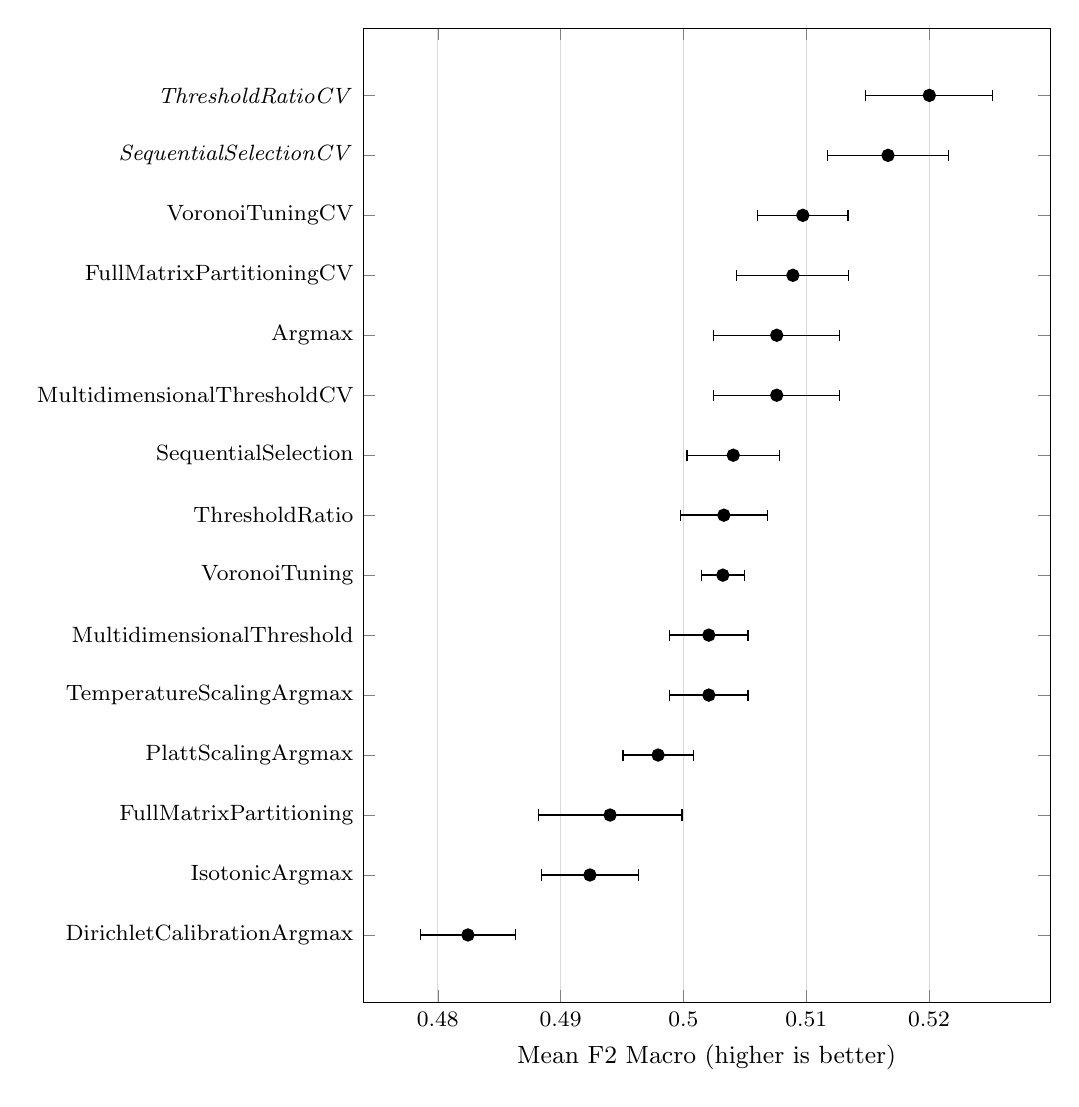
\begin{tikzpicture}
\begin{axis}[
    width=0.85\textwidth, height=13.95cm,
    xlabel={Mean F2 Macro (higher is better)},
    symbolic y coords={{ThresholdRatioCV},{SequentialSelectionCV},{VoronoiTuningCV},{FullMatrixPartitioningCV},{Argmax},{MultidimensionalThresholdCV},{SequentialSelection},{ThresholdRatio},{VoronoiTuning},{MultidimensionalThreshold},{TemperatureScalingArgmax},{PlattScalingArgmax},{FullMatrixPartitioning},{IsotonicArgmax},{DirichletCalibrationArgmax}},
    ytick={{ThresholdRatioCV},{SequentialSelectionCV},{VoronoiTuningCV},{FullMatrixPartitioningCV},{Argmax},{MultidimensionalThresholdCV},{SequentialSelection},{ThresholdRatio},{VoronoiTuning},{MultidimensionalThreshold},{TemperatureScalingArgmax},{PlattScalingArgmax},{FullMatrixPartitioning},{IsotonicArgmax},{DirichletCalibrationArgmax}},
    yticklabels={\textit{ThresholdRatioCV},\textit{SequentialSelectionCV},VoronoiTuningCV,FullMatrixPartitioningCV,Argmax,MultidimensionalThresholdCV,SequentialSelection,ThresholdRatio,VoronoiTuning,MultidimensionalThreshold,TemperatureScalingArgmax,PlattScalingArgmax,FullMatrixPartitioning,IsotonicArgmax,DirichletCalibrationArgmax},
    y dir=reverse,
    enlarge y limits=0.08,
    xmajorgrids=true,
    major grid style={draw=black!15, line width=0.3pt},
    scaled x ticks=false,
    xticklabel style={/pgf/number format/fixed, /pgf/number format/precision=3},
    tick label style={font=\footnotesize},
    label style={font=\small},
    every axis plot/.append style={thick},
]
\addplot[only marks, mark=*, mark size=2pt, color=black, error bars/x dir=both, error bars/x explicit, error bars/error bar style={color=black, line width=0.5pt}] coordinates { (0.520024,{ThresholdRatioCV}) +- (0.00517868,0) };
\addplot[only marks, mark=*, mark size=2pt, color=black, error bars/x dir=both, error bars/x explicit, error bars/error bar style={color=black, line width=0.5pt}] coordinates { (0.51666,{SequentialSelectionCV}) +- (0.00495574,0) };
\addplot[only marks, mark=*, mark size=2pt, color=black, error bars/x dir=both, error bars/x explicit, error bars/error bar style={color=black, line width=0.5pt}] coordinates { (0.509723,{VoronoiTuningCV}) +- (0.0036767,0) };
\addplot[only marks, mark=*, mark size=2pt, color=black, error bars/x dir=both, error bars/x explicit, error bars/error bar style={color=black, line width=0.5pt}] coordinates { (0.508913,{FullMatrixPartitioningCV}) +- (0.00455732,0) };
\addplot[only marks, mark=*, mark size=2pt, color=black, error bars/x dir=both, error bars/x explicit, error bars/error bar style={color=black, line width=0.5pt}] coordinates { (0.507598,{Argmax}) +- (0.00512521,0) };
\addplot[only marks, mark=*, mark size=2pt, color=black, error bars/x dir=both, error bars/x explicit, error bars/error bar style={color=black, line width=0.5pt}] coordinates { (0.507598,{MultidimensionalThresholdCV}) +- (0.00512521,0) };
\addplot[only marks, mark=*, mark size=2pt, color=black, error bars/x dir=both, error bars/x explicit, error bars/error bar style={color=black, line width=0.5pt}] coordinates { (0.504059,{SequentialSelection}) +- (0.00376794,0) };
\addplot[only marks, mark=*, mark size=2pt, color=black, error bars/x dir=both, error bars/x explicit, error bars/error bar style={color=black, line width=0.5pt}] coordinates { (0.503293,{ThresholdRatio}) +- (0.00352692,0) };
\addplot[only marks, mark=*, mark size=2pt, color=black, error bars/x dir=both, error bars/x explicit, error bars/error bar style={color=black, line width=0.5pt}] coordinates { (0.503212,{VoronoiTuning}) +- (0.00173639,0) };
\addplot[only marks, mark=*, mark size=2pt, color=black, error bars/x dir=both, error bars/x explicit, error bars/error bar style={color=black, line width=0.5pt}] coordinates { (0.502071,{MultidimensionalThreshold}) +- (0.00318547,0) };
\addplot[only marks, mark=*, mark size=2pt, color=black, error bars/x dir=both, error bars/x explicit, error bars/error bar style={color=black, line width=0.5pt}] coordinates { (0.502071,{TemperatureScalingArgmax}) +- (0.00318547,0) };
\addplot[only marks, mark=*, mark size=2pt, color=black, error bars/x dir=both, error bars/x explicit, error bars/error bar style={color=black, line width=0.5pt}] coordinates { (0.49794,{PlattScalingArgmax}) +- (0.00286004,0) };
\addplot[only marks, mark=*, mark size=2pt, color=black, error bars/x dir=both, error bars/x explicit, error bars/error bar style={color=black, line width=0.5pt}] coordinates { (0.494029,{FullMatrixPartitioning}) +- (0.00585333,0) };
\addplot[only marks, mark=*, mark size=2pt, color=black, error bars/x dir=both, error bars/x explicit, error bars/error bar style={color=black, line width=0.5pt}] coordinates { (0.492389,{IsotonicArgmax}) +- (0.00395195,0) };
\addplot[only marks, mark=*, mark size=2pt, color=black, error bars/x dir=both, error bars/x explicit, error bars/error bar style={color=black, line width=0.5pt}] coordinates { (0.482454,{DirichletCalibrationArgmax}) +- (0.00386869,0) };
\end{axis}
\end{tikzpicture}%
}
\caption{fot\_proving: F2 Macro on LGBM (higher is better). Each dot is a strategy's mean over ten seeds with a $\pm 1$ SE horizontal bar; rows are sorted by mean, and the best strategy and any whose interval overlaps it are italicized.}%
\label{fig:ci-fot_proving-f2_macro}
\end{figure}


Figures~\ref{fig:win-counts-multiclass-cost} and~\ref{fig:win-counts-multiclass-max} give the per-strategy win and tie rates under the $\pm 1$ SE overlap rule, broken out by base classifier and by dataset size and imbalance bucket; the figure captions document the reading convention and the bootstrap half-width. The dominant pattern on both objective groups is the gap between each cross-validated tuning variant and its single-split counterpart. DirichletCalibrationArgmax sits near the floor on every slice.

% Auto-generated by experiments.analysis.generate_win_counts --- do not edit.
\begin{figure}[H]
\centering
\adjustbox{max width=\textwidth}{%
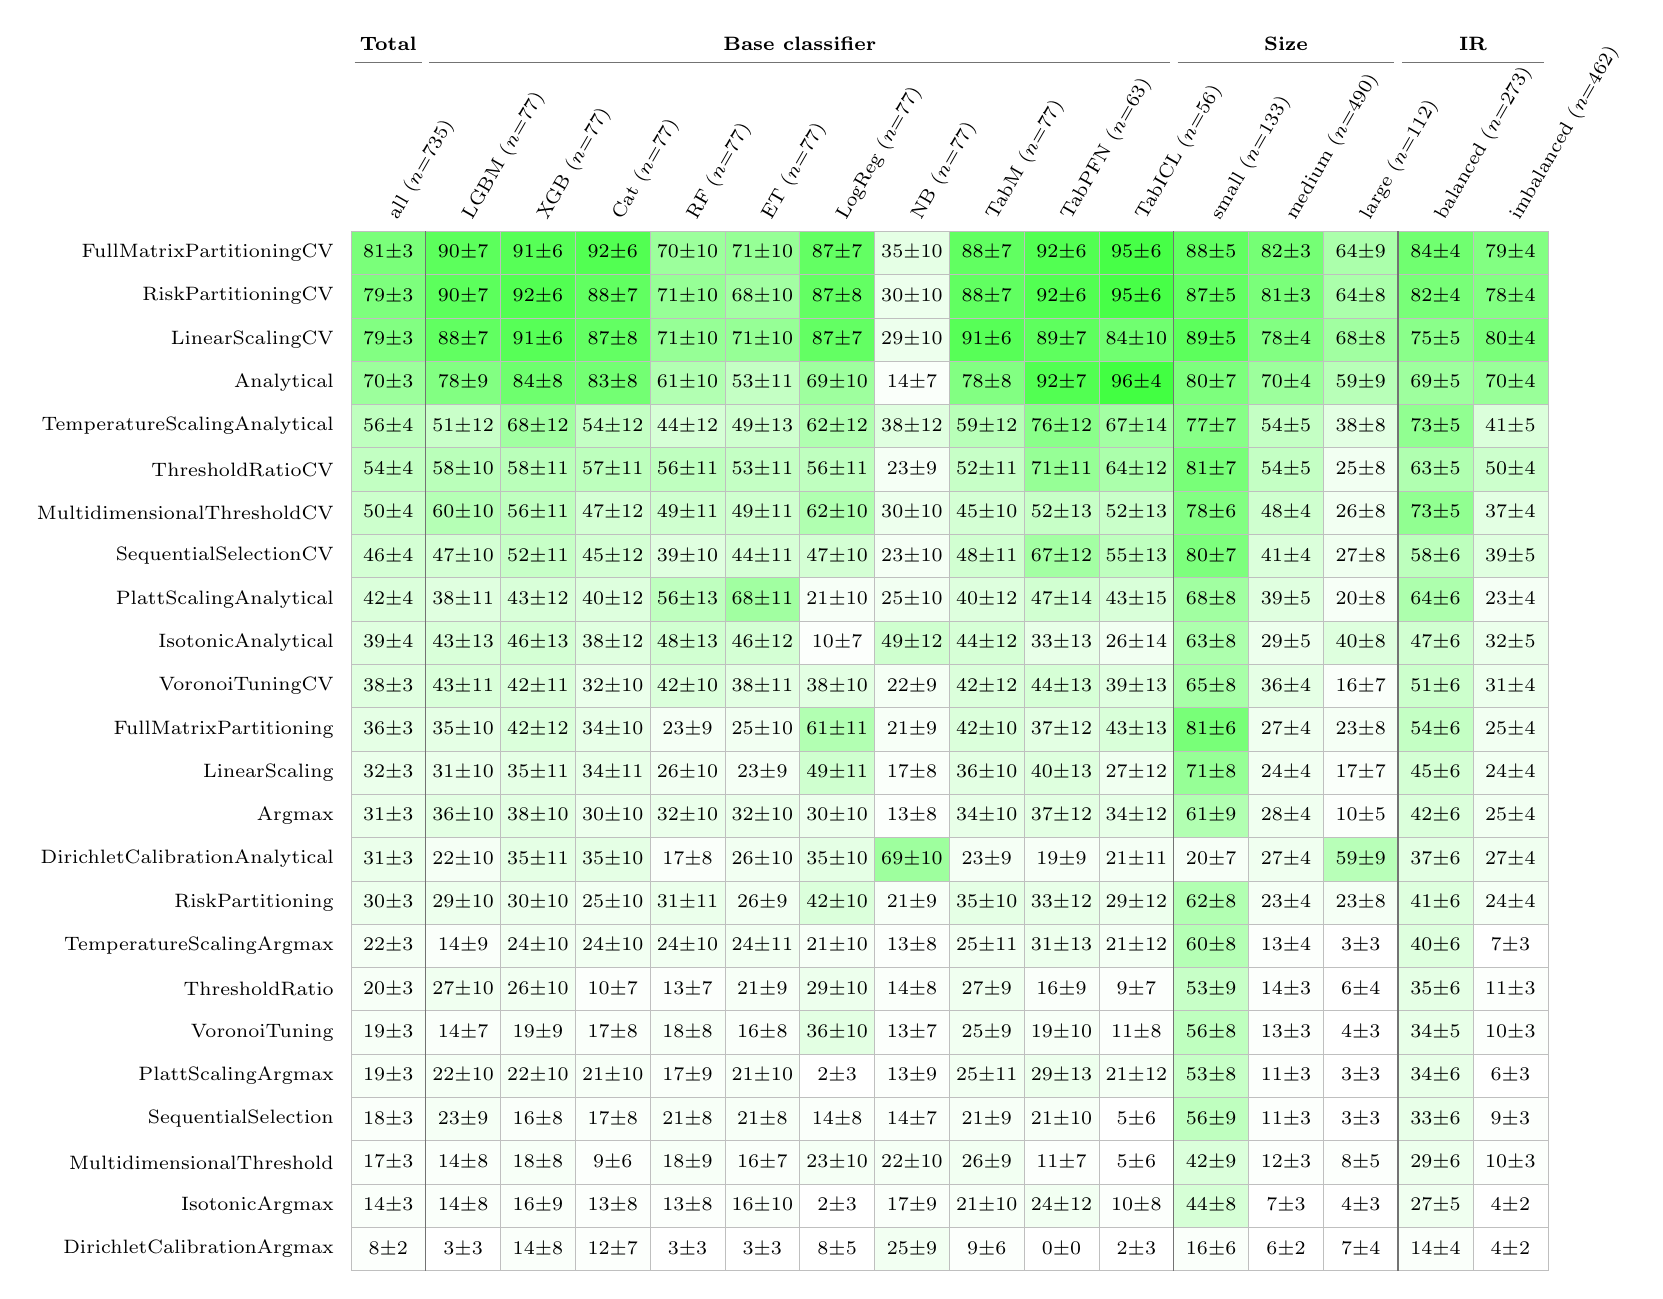
\begin{tikzpicture}[
    x=0.95cm, y=0.55cm,
    cell/.style={rectangle, draw=black!25, line width=0.2pt,
        minimum width=0.95cm, minimum height=0.55cm,
        anchor=center, font=\scriptsize, inner sep=0pt},
    rowlbl/.style={font=\scriptsize, anchor=east},
    collbl/.style={font=\scriptsize, anchor=west, rotate=60},
    grouplbl/.style={font=\scriptsize\bfseries, anchor=south},
    sep/.style={draw=black!55, line width=0.5pt},
]
\node[cell, fill=green!52] at (1, 24) {$81{\pm}3$};
\node[cell, fill=green!64] at (2, 24) {$90{\pm}7$};
\node[cell, fill=green!66] at (3, 24) {$91{\pm}6$};
\node[cell, fill=green!68] at (4, 24) {$92{\pm}6$};
\node[cell, fill=green!39] at (5, 24) {$70{\pm}10$};
\node[cell, fill=green!41] at (6, 24) {$71{\pm}10$};
\node[cell, fill=green!61] at (7, 24) {$87{\pm}7$};
\node[cell, fill=green!10] at (8, 24) {$35{\pm}10$};
\node[cell, fill=green!62] at (9, 24) {$88{\pm}7$};
\node[cell, fill=green!68] at (10, 24) {$92{\pm}6$};
\node[cell, fill=green!72] at (11, 24) {$95{\pm}6$};
\node[cell, fill=green!62] at (12, 24) {$88{\pm}5$};
\node[cell, fill=green!54] at (13, 24) {$82{\pm}3$};
\node[cell, fill=green!33] at (14, 24) {$64{\pm}9$};
\node[cell, fill=green!56] at (15, 24) {$84{\pm}4$};
\node[cell, fill=green!49] at (16, 24) {$79{\pm}4$};
\node[cell, fill=green!51] at (1, 23) {$79{\pm}3$};
\node[cell, fill=green!64] at (2, 23) {$90{\pm}7$};
\node[cell, fill=green!68] at (3, 23) {$92{\pm}6$};
\node[cell, fill=green!62] at (4, 23) {$88{\pm}7$};
\node[cell, fill=green!41] at (5, 23) {$71{\pm}10$};
\node[cell, fill=green!36] at (6, 23) {$68{\pm}10$};
\node[cell, fill=green!61] at (7, 23) {$87{\pm}8$};
\node[cell, fill=green!7] at (8, 23) {$30{\pm}10$};
\node[cell, fill=green!62] at (9, 23) {$88{\pm}7$};
\node[cell, fill=green!68] at (10, 23) {$92{\pm}6$};
\node[cell, fill=green!72] at (11, 23) {$95{\pm}6$};
\node[cell, fill=green!61] at (12, 23) {$87{\pm}5$};
\node[cell, fill=green!52] at (13, 23) {$81{\pm}3$};
\node[cell, fill=green!33] at (14, 23) {$64{\pm}8$};
\node[cell, fill=green!53] at (15, 23) {$82{\pm}4$};
\node[cell, fill=green!49] at (16, 23) {$78{\pm}4$};
\node[cell, fill=green!49] at (1, 22) {$79{\pm}3$};
\node[cell, fill=green!62] at (2, 22) {$88{\pm}7$};
\node[cell, fill=green!66] at (3, 22) {$91{\pm}6$};
\node[cell, fill=green!61] at (4, 22) {$87{\pm}8$};
\node[cell, fill=green!41] at (5, 22) {$71{\pm}10$};
\node[cell, fill=green!41] at (6, 22) {$71{\pm}10$};
\node[cell, fill=green!61] at (7, 22) {$87{\pm}7$};
\node[cell, fill=green!7] at (8, 22) {$29{\pm}10$};
\node[cell, fill=green!66] at (9, 22) {$91{\pm}6$};
\node[cell, fill=green!63] at (10, 22) {$89{\pm}7$};
\node[cell, fill=green!56] at (11, 22) {$84{\pm}10$};
\node[cell, fill=green!64] at (12, 22) {$89{\pm}5$};
\node[cell, fill=green!49] at (13, 22) {$78{\pm}4$};
\node[cell, fill=green!37] at (14, 22) {$68{\pm}8$};
\node[cell, fill=green!46] at (15, 22) {$75{\pm}5$};
\node[cell, fill=green!52] at (16, 22) {$80{\pm}4$};
\node[cell, fill=green!39] at (1, 21) {$70{\pm}3$};
\node[cell, fill=green!49] at (2, 21) {$78{\pm}9$};
\node[cell, fill=green!57] at (3, 21) {$84{\pm}8$};
\node[cell, fill=green!55] at (4, 21) {$83{\pm}8$};
\node[cell, fill=green!30] at (5, 21) {$61{\pm}10$};
\node[cell, fill=green!23] at (6, 21) {$53{\pm}11$};
\node[cell, fill=green!38] at (7, 21) {$69{\pm}10$};
\node[cell, fill=green!2] at (8, 21) {$14{\pm}7$};
\node[cell, fill=green!49] at (9, 21) {$78{\pm}8$};
\node[cell, fill=green!68] at (10, 21) {$92{\pm}7$};
\node[cell, fill=green!74] at (11, 21) {$96{\pm}4$};
\node[cell, fill=green!51] at (12, 21) {$80{\pm}7$};
\node[cell, fill=green!39] at (13, 21) {$70{\pm}4$};
\node[cell, fill=green!28] at (14, 21) {$59{\pm}9$};
\node[cell, fill=green!38] at (15, 21) {$69{\pm}5$};
\node[cell, fill=green!40] at (16, 21) {$70{\pm}4$};
\node[cell, fill=green!25] at (1, 20) {$56{\pm}4$};
\node[cell, fill=green!21] at (2, 20) {$51{\pm}12$};
\node[cell, fill=green!37] at (3, 20) {$68{\pm}12$};
\node[cell, fill=green!23] at (4, 20) {$54{\pm}12$};
\node[cell, fill=green!16] at (5, 20) {$44{\pm}12$};
\node[cell, fill=green!19] at (6, 20) {$49{\pm}13$};
\node[cell, fill=green!31] at (7, 20) {$62{\pm}12$};
\node[cell, fill=green!12] at (8, 20) {$38{\pm}12$};
\node[cell, fill=green!28] at (9, 20) {$59{\pm}12$};
\node[cell, fill=green!46] at (10, 20) {$76{\pm}12$};
\node[cell, fill=green!36] at (11, 20) {$67{\pm}14$};
\node[cell, fill=green!47] at (12, 20) {$77{\pm}7$};
\node[cell, fill=green!23] at (13, 20) {$54{\pm}5$};
\node[cell, fill=green!11] at (14, 20) {$38{\pm}8$};
\node[cell, fill=green!43] at (15, 20) {$73{\pm}5$};
\node[cell, fill=green!14] at (16, 20) {$41{\pm}5$};
\node[cell, fill=green!24] at (1, 19) {$54{\pm}4$};
\node[cell, fill=green!27] at (2, 19) {$58{\pm}10$};
\node[cell, fill=green!27] at (3, 19) {$58{\pm}11$};
\node[cell, fill=green!26] at (4, 19) {$57{\pm}11$};
\node[cell, fill=green!25] at (5, 19) {$56{\pm}11$};
\node[cell, fill=green!23] at (6, 19) {$53{\pm}11$};
\node[cell, fill=green!25] at (7, 19) {$56{\pm}11$};
\node[cell, fill=green!4] at (8, 19) {$23{\pm}9$};
\node[cell, fill=green!22] at (9, 19) {$52{\pm}11$};
\node[cell, fill=green!41] at (10, 19) {$71{\pm}11$};
\node[cell, fill=green!33] at (11, 19) {$64{\pm}12$};
\node[cell, fill=green!53] at (12, 19) {$81{\pm}7$};
\node[cell, fill=green!23] at (13, 19) {$54{\pm}5$};
\node[cell, fill=green!5] at (14, 19) {$25{\pm}8$};
\node[cell, fill=green!31] at (15, 19) {$63{\pm}5$};
\node[cell, fill=green!20] at (16, 19) {$50{\pm}4$};
\node[cell, fill=green!20] at (1, 18) {$50{\pm}4$};
\node[cell, fill=green!29] at (2, 18) {$60{\pm}10$};
\node[cell, fill=green!25] at (3, 18) {$56{\pm}11$};
\node[cell, fill=green!17] at (4, 18) {$47{\pm}12$};
\node[cell, fill=green!19] at (5, 18) {$49{\pm}11$};
\node[cell, fill=green!19] at (6, 18) {$49{\pm}11$};
\node[cell, fill=green!31] at (7, 18) {$62{\pm}10$};
\node[cell, fill=green!7] at (8, 18) {$30{\pm}10$};
\node[cell, fill=green!17] at (9, 18) {$45{\pm}10$};
\node[cell, fill=green!22] at (10, 18) {$52{\pm}13$};
\node[cell, fill=green!21] at (11, 18) {$52{\pm}13$};
\node[cell, fill=green!49] at (12, 18) {$78{\pm}6$};
\node[cell, fill=green!19] at (13, 18) {$48{\pm}4$};
\node[cell, fill=green!5] at (14, 18) {$26{\pm}8$};
\node[cell, fill=green!43] at (15, 18) {$73{\pm}5$};
\node[cell, fill=green!11] at (16, 18) {$37{\pm}4$};
\node[cell, fill=green!17] at (1, 17) {$46{\pm}4$};
\node[cell, fill=green!17] at (2, 17) {$47{\pm}10$};
\node[cell, fill=green!22] at (3, 17) {$52{\pm}11$};
\node[cell, fill=green!17] at (4, 17) {$45{\pm}12$};
\node[cell, fill=green!12] at (5, 17) {$39{\pm}10$};
\node[cell, fill=green!16] at (6, 17) {$44{\pm}11$};
\node[cell, fill=green!17] at (7, 17) {$47{\pm}10$};
\node[cell, fill=green!4] at (8, 17) {$23{\pm}10$};
\node[cell, fill=green!18] at (9, 17) {$48{\pm}11$};
\node[cell, fill=green!36] at (10, 17) {$67{\pm}12$};
\node[cell, fill=green!25] at (11, 17) {$55{\pm}13$};
\node[cell, fill=green!51] at (12, 17) {$80{\pm}7$};
\node[cell, fill=green!14] at (13, 17) {$41{\pm}4$};
\node[cell, fill=green!6] at (14, 17) {$27{\pm}8$};
\node[cell, fill=green!26] at (15, 17) {$58{\pm}6$};
\node[cell, fill=green!12] at (16, 17) {$39{\pm}5$};
\node[cell, fill=green!14] at (1, 16) {$42{\pm}4$};
\node[cell, fill=green!12] at (2, 16) {$38{\pm}11$};
\node[cell, fill=green!15] at (3, 16) {$43{\pm}12$};
\node[cell, fill=green!13] at (4, 16) {$40{\pm}12$};
\node[cell, fill=green!25] at (5, 16) {$56{\pm}13$};
\node[cell, fill=green!37] at (6, 16) {$68{\pm}11$};
\node[cell, fill=green!3] at (7, 16) {$21{\pm}10$};
\node[cell, fill=green!5] at (8, 16) {$25{\pm}10$};
\node[cell, fill=green!13] at (9, 16) {$40{\pm}12$};
\node[cell, fill=green!18] at (10, 16) {$47{\pm}14$};
\node[cell, fill=green!15] at (11, 16) {$43{\pm}15$};
\node[cell, fill=green!37] at (12, 16) {$68{\pm}8$};
\node[cell, fill=green!12] at (13, 16) {$39{\pm}5$};
\node[cell, fill=green!3] at (14, 16) {$20{\pm}8$};
\node[cell, fill=green!32] at (15, 16) {$64{\pm}6$};
\node[cell, fill=green!4] at (16, 16) {$23{\pm}4$};
\node[cell, fill=green!12] at (1, 15) {$39{\pm}4$};
\node[cell, fill=green!15] at (2, 15) {$43{\pm}13$};
\node[cell, fill=green!17] at (3, 15) {$46{\pm}13$};
\node[cell, fill=green!12] at (4, 15) {$38{\pm}12$};
\node[cell, fill=green!18] at (5, 15) {$48{\pm}13$};
\node[cell, fill=green!17] at (6, 15) {$46{\pm}12$};
\node[cell, fill=green!1] at (7, 15) {$10{\pm}7$};
\node[cell, fill=green!19] at (8, 15) {$49{\pm}12$};
\node[cell, fill=green!16] at (9, 15) {$44{\pm}12$};
\node[cell, fill=green!9] at (10, 15) {$33{\pm}13$};
\node[cell, fill=green!5] at (11, 15) {$26{\pm}14$};
\node[cell, fill=green!32] at (12, 15) {$63{\pm}8$};
\node[cell, fill=green!7] at (13, 15) {$29{\pm}5$};
\node[cell, fill=green!13] at (14, 15) {$40{\pm}8$};
\node[cell, fill=green!18] at (15, 15) {$47{\pm}6$};
\node[cell, fill=green!8] at (16, 15) {$32{\pm}5$};
\node[cell, fill=green!12] at (1, 14) {$38{\pm}3$};
\node[cell, fill=green!15] at (2, 14) {$43{\pm}11$};
\node[cell, fill=green!14] at (3, 14) {$42{\pm}11$};
\node[cell, fill=green!8] at (4, 14) {$32{\pm}10$};
\node[cell, fill=green!14] at (5, 14) {$42{\pm}10$};
\node[cell, fill=green!11] at (6, 14) {$38{\pm}11$};
\node[cell, fill=green!11] at (7, 14) {$38{\pm}10$};
\node[cell, fill=green!4] at (8, 14) {$22{\pm}9$};
\node[cell, fill=green!14] at (9, 14) {$42{\pm}12$};
\node[cell, fill=green!16] at (10, 14) {$44{\pm}13$};
\node[cell, fill=green!12] at (11, 14) {$39{\pm}13$};
\node[cell, fill=green!34] at (12, 14) {$65{\pm}8$};
\node[cell, fill=green!10] at (13, 14) {$36{\pm}4$};
\node[cell, fill=green!2] at (14, 14) {$16{\pm}7$};
\node[cell, fill=green!20] at (15, 14) {$51{\pm}6$};
\node[cell, fill=green!7] at (16, 14) {$31{\pm}4$};
\node[cell, fill=green!10] at (1, 13) {$36{\pm}3$};
\node[cell, fill=green!10] at (2, 13) {$35{\pm}10$};
\node[cell, fill=green!14] at (3, 13) {$42{\pm}12$};
\node[cell, fill=green!9] at (4, 13) {$34{\pm}10$};
\node[cell, fill=green!4] at (5, 13) {$23{\pm}9$};
\node[cell, fill=green!5] at (6, 13) {$25{\pm}10$};
\node[cell, fill=green!30] at (7, 13) {$61{\pm}11$};
\node[cell, fill=green!3] at (8, 13) {$21{\pm}9$};
\node[cell, fill=green!14] at (9, 13) {$42{\pm}10$};
\node[cell, fill=green!11] at (10, 13) {$37{\pm}12$};
\node[cell, fill=green!15] at (11, 13) {$43{\pm}13$};
\node[cell, fill=green!53] at (12, 13) {$81{\pm}6$};
\node[cell, fill=green!6] at (13, 13) {$27{\pm}4$};
\node[cell, fill=green!4] at (14, 13) {$23{\pm}8$};
\node[cell, fill=green!23] at (15, 13) {$54{\pm}6$};
\node[cell, fill=green!5] at (16, 13) {$25{\pm}4$};
\node[cell, fill=green!8] at (1, 12) {$32{\pm}3$};
\node[cell, fill=green!8] at (2, 12) {$31{\pm}10$};
\node[cell, fill=green!10] at (3, 12) {$35{\pm}11$};
\node[cell, fill=green!9] at (4, 12) {$34{\pm}11$};
\node[cell, fill=green!5] at (5, 12) {$26{\pm}10$};
\node[cell, fill=green!4] at (6, 12) {$23{\pm}9$};
\node[cell, fill=green!19] at (7, 12) {$49{\pm}11$};
\node[cell, fill=green!2] at (8, 12) {$17{\pm}8$};
\node[cell, fill=green!11] at (9, 12) {$36{\pm}10$};
\node[cell, fill=green!13] at (10, 12) {$40{\pm}13$};
\node[cell, fill=green!6] at (11, 12) {$27{\pm}12$};
\node[cell, fill=green!41] at (12, 12) {$71{\pm}8$};
\node[cell, fill=green!5] at (13, 12) {$24{\pm}4$};
\node[cell, fill=green!2] at (14, 12) {$17{\pm}7$};
\node[cell, fill=green!17] at (15, 12) {$45{\pm}6$};
\node[cell, fill=green!5] at (16, 12) {$24{\pm}4$};
\node[cell, fill=green!8] at (1, 11) {$31{\pm}3$};
\node[cell, fill=green!11] at (2, 11) {$36{\pm}10$};
\node[cell, fill=green!11] at (3, 11) {$38{\pm}10$};
\node[cell, fill=green!7] at (4, 11) {$30{\pm}10$};
\node[cell, fill=green!8] at (5, 11) {$32{\pm}10$};
\node[cell, fill=green!8] at (6, 11) {$32{\pm}10$};
\node[cell, fill=green!7] at (7, 11) {$30{\pm}10$};
\node[cell, fill=green!1] at (8, 11) {$13{\pm}8$};
\node[cell, fill=green!9] at (9, 11) {$34{\pm}10$};
\node[cell, fill=green!11] at (10, 11) {$37{\pm}12$};
\node[cell, fill=green!9] at (11, 11) {$34{\pm}12$};
\node[cell, fill=green!30] at (12, 11) {$61{\pm}9$};
\node[cell, fill=green!6] at (13, 11) {$28{\pm}4$};
\node[cell, fill=green!1] at (14, 11) {$10{\pm}5$};
\node[cell, fill=green!14] at (15, 11) {$42{\pm}6$};
\node[cell, fill=green!5] at (16, 11) {$25{\pm}4$};
\node[cell, fill=green!8] at (1, 10) {$31{\pm}3$};
\node[cell, fill=green!4] at (2, 10) {$22{\pm}10$};
\node[cell, fill=green!10] at (3, 10) {$35{\pm}11$};
\node[cell, fill=green!10] at (4, 10) {$35{\pm}10$};
\node[cell, fill=green!2] at (5, 10) {$17{\pm}8$};
\node[cell, fill=green!5] at (6, 10) {$26{\pm}10$};
\node[cell, fill=green!10] at (7, 10) {$35{\pm}10$};
\node[cell, fill=green!38] at (8, 10) {$69{\pm}10$};
\node[cell, fill=green!4] at (9, 10) {$23{\pm}9$};
\node[cell, fill=green!3] at (10, 10) {$19{\pm}9$};
\node[cell, fill=green!4] at (11, 10) {$21{\pm}11$};
\node[cell, fill=green!3] at (12, 10) {$20{\pm}7$};
\node[cell, fill=green!6] at (13, 10) {$27{\pm}4$};
\node[cell, fill=green!28] at (14, 10) {$59{\pm}9$};
\node[cell, fill=green!11] at (15, 10) {$37{\pm}6$};
\node[cell, fill=green!6] at (16, 10) {$27{\pm}4$};
\node[cell, fill=green!7] at (1, 9) {$30{\pm}3$};
\node[cell, fill=green!7] at (2, 9) {$29{\pm}10$};
\node[cell, fill=green!7] at (3, 9) {$30{\pm}10$};
\node[cell, fill=green!5] at (4, 9) {$25{\pm}10$};
\node[cell, fill=green!8] at (5, 9) {$31{\pm}11$};
\node[cell, fill=green!5] at (6, 9) {$26{\pm}9$};
\node[cell, fill=green!14] at (7, 9) {$42{\pm}10$};
\node[cell, fill=green!3] at (8, 9) {$21{\pm}9$};
\node[cell, fill=green!10] at (9, 9) {$35{\pm}10$};
\node[cell, fill=green!9] at (10, 9) {$33{\pm}12$};
\node[cell, fill=green!7] at (11, 9) {$29{\pm}12$};
\node[cell, fill=green!30] at (12, 9) {$62{\pm}8$};
\node[cell, fill=green!4] at (13, 9) {$23{\pm}4$};
\node[cell, fill=green!4] at (14, 9) {$23{\pm}8$};
\node[cell, fill=green!13] at (15, 9) {$41{\pm}6$};
\node[cell, fill=green!4] at (16, 9) {$24{\pm}4$};
\node[cell, fill=green!4] at (1, 8) {$22{\pm}3$};
\node[cell, fill=green!2] at (2, 8) {$14{\pm}9$};
\node[cell, fill=green!5] at (3, 8) {$24{\pm}10$};
\node[cell, fill=green!5] at (4, 8) {$24{\pm}10$};
\node[cell, fill=green!5] at (5, 8) {$24{\pm}10$};
\node[cell, fill=green!5] at (6, 8) {$24{\pm}11$};
\node[cell, fill=green!3] at (7, 8) {$21{\pm}10$};
\node[cell, fill=green!1] at (8, 8) {$13{\pm}8$};
\node[cell, fill=green!5] at (9, 8) {$25{\pm}11$};
\node[cell, fill=green!7] at (10, 8) {$31{\pm}13$};
\node[cell, fill=green!4] at (11, 8) {$21{\pm}12$};
\node[cell, fill=green!29] at (12, 8) {$60{\pm}8$};
\node[cell, fill=green!1] at (13, 8) {$13{\pm}4$};
\node[cell, fill=green!0] at (14, 8) {$3{\pm}3$};
\node[cell, fill=green!13] at (15, 8) {$40{\pm}6$};
\node[cell, fill=green!0] at (16, 8) {$7{\pm}3$};
\node[cell, fill=green!3] at (1, 7) {$20{\pm}3$};
\node[cell, fill=green!6] at (2, 7) {$27{\pm}10$};
\node[cell, fill=green!5] at (3, 7) {$26{\pm}10$};
\node[cell, fill=green!1] at (4, 7) {$10{\pm}7$};
\node[cell, fill=green!1] at (5, 7) {$13{\pm}7$};
\node[cell, fill=green!3] at (6, 7) {$21{\pm}9$};
\node[cell, fill=green!7] at (7, 7) {$29{\pm}10$};
\node[cell, fill=green!2] at (8, 7) {$14{\pm}8$};
\node[cell, fill=green!6] at (9, 7) {$27{\pm}9$};
\node[cell, fill=green!2] at (10, 7) {$16{\pm}9$};
\node[cell, fill=green!1] at (11, 7) {$9{\pm}7$};
\node[cell, fill=green!22] at (12, 7) {$53{\pm}9$};
\node[cell, fill=green!1] at (13, 7) {$14{\pm}3$};
\node[cell, fill=green!0] at (14, 7) {$6{\pm}4$};
\node[cell, fill=green!10] at (15, 7) {$35{\pm}6$};
\node[cell, fill=green!1] at (16, 7) {$11{\pm}3$};
\node[cell, fill=green!3] at (1, 6) {$19{\pm}3$};
\node[cell, fill=green!2] at (2, 6) {$14{\pm}7$};
\node[cell, fill=green!3] at (3, 6) {$19{\pm}9$};
\node[cell, fill=green!2] at (4, 6) {$17{\pm}8$};
\node[cell, fill=green!3] at (5, 6) {$18{\pm}8$};
\node[cell, fill=green!2] at (6, 6) {$16{\pm}8$};
\node[cell, fill=green!11] at (7, 6) {$36{\pm}10$};
\node[cell, fill=green!1] at (8, 6) {$13{\pm}7$};
\node[cell, fill=green!5] at (9, 6) {$25{\pm}9$};
\node[cell, fill=green!3] at (10, 6) {$19{\pm}10$};
\node[cell, fill=green!1] at (11, 6) {$11{\pm}8$};
\node[cell, fill=green!25] at (12, 6) {$56{\pm}8$};
\node[cell, fill=green!1] at (13, 6) {$13{\pm}3$};
\node[cell, fill=green!0] at (14, 6) {$4{\pm}3$};
\node[cell, fill=green!9] at (15, 6) {$34{\pm}5$};
\node[cell, fill=green!1] at (16, 6) {$10{\pm}3$};
\node[cell, fill=green!3] at (1, 5) {$19{\pm}3$};
\node[cell, fill=green!4] at (2, 5) {$22{\pm}10$};
\node[cell, fill=green!4] at (3, 5) {$22{\pm}10$};
\node[cell, fill=green!3] at (4, 5) {$21{\pm}10$};
\node[cell, fill=green!2] at (5, 5) {$17{\pm}9$};
\node[cell, fill=green!3] at (6, 5) {$21{\pm}10$};
\node[cell, fill=green!0] at (7, 5) {$2{\pm}3$};
\node[cell, fill=green!1] at (8, 5) {$13{\pm}9$};
\node[cell, fill=green!5] at (9, 5) {$25{\pm}11$};
\node[cell, fill=green!7] at (10, 5) {$29{\pm}13$};
\node[cell, fill=green!4] at (11, 5) {$21{\pm}12$};
\node[cell, fill=green!22] at (12, 5) {$53{\pm}8$};
\node[cell, fill=green!1] at (13, 5) {$11{\pm}3$};
\node[cell, fill=green!0] at (14, 5) {$3{\pm}3$};
\node[cell, fill=green!9] at (15, 5) {$34{\pm}6$};
\node[cell, fill=green!0] at (16, 5) {$6{\pm}3$};
\node[cell, fill=green!2] at (1, 4) {$18{\pm}3$};
\node[cell, fill=green!4] at (2, 4) {$23{\pm}9$};
\node[cell, fill=green!2] at (3, 4) {$16{\pm}8$};
\node[cell, fill=green!2] at (4, 4) {$17{\pm}8$};
\node[cell, fill=green!3] at (5, 4) {$21{\pm}8$};
\node[cell, fill=green!3] at (6, 4) {$21{\pm}8$};
\node[cell, fill=green!2] at (7, 4) {$14{\pm}8$};
\node[cell, fill=green!2] at (8, 4) {$14{\pm}7$};
\node[cell, fill=green!3] at (9, 4) {$21{\pm}9$};
\node[cell, fill=green!3] at (10, 4) {$21{\pm}10$};
\node[cell, fill=green!0] at (11, 4) {$5{\pm}6$};
\node[cell, fill=green!25] at (12, 4) {$56{\pm}9$};
\node[cell, fill=green!1] at (13, 4) {$11{\pm}3$};
\node[cell, fill=green!0] at (14, 4) {$3{\pm}3$};
\node[cell, fill=green!9] at (15, 4) {$33{\pm}6$};
\node[cell, fill=green!1] at (16, 4) {$9{\pm}3$};
\node[cell, fill=green!2] at (1, 3) {$17{\pm}3$};
\node[cell, fill=green!2] at (2, 3) {$14{\pm}8$};
\node[cell, fill=green!3] at (3, 3) {$18{\pm}8$};
\node[cell, fill=green!1] at (4, 3) {$9{\pm}6$};
\node[cell, fill=green!3] at (5, 3) {$18{\pm}9$};
\node[cell, fill=green!2] at (6, 3) {$16{\pm}7$};
\node[cell, fill=green!4] at (7, 3) {$23{\pm}10$};
\node[cell, fill=green!4] at (8, 3) {$22{\pm}10$};
\node[cell, fill=green!5] at (9, 3) {$26{\pm}9$};
\node[cell, fill=green!1] at (10, 3) {$11{\pm}7$};
\node[cell, fill=green!0] at (11, 3) {$5{\pm}6$};
\node[cell, fill=green!14] at (12, 3) {$42{\pm}9$};
\node[cell, fill=green!1] at (13, 3) {$12{\pm}3$};
\node[cell, fill=green!1] at (14, 3) {$8{\pm}5$};
\node[cell, fill=green!7] at (15, 3) {$29{\pm}6$};
\node[cell, fill=green!1] at (16, 3) {$10{\pm}3$};
\node[cell, fill=green!2] at (1, 2) {$14{\pm}3$};
\node[cell, fill=green!2] at (2, 2) {$14{\pm}8$};
\node[cell, fill=green!2] at (3, 2) {$16{\pm}9$};
\node[cell, fill=green!1] at (4, 2) {$13{\pm}8$};
\node[cell, fill=green!1] at (5, 2) {$13{\pm}8$};
\node[cell, fill=green!2] at (6, 2) {$16{\pm}10$};
\node[cell, fill=green!0] at (7, 2) {$2{\pm}3$};
\node[cell, fill=green!2] at (8, 2) {$17{\pm}9$};
\node[cell, fill=green!3] at (9, 2) {$21{\pm}10$};
\node[cell, fill=green!5] at (10, 2) {$24{\pm}12$};
\node[cell, fill=green!1] at (11, 2) {$10{\pm}8$};
\node[cell, fill=green!16] at (12, 2) {$44{\pm}8$};
\node[cell, fill=green!0] at (13, 2) {$7{\pm}3$};
\node[cell, fill=green!0] at (14, 2) {$4{\pm}3$};
\node[cell, fill=green!6] at (15, 2) {$27{\pm}5$};
\node[cell, fill=green!0] at (16, 2) {$4{\pm}2$};
\node[cell, fill=green!1] at (1, 1) {$8{\pm}2$};
\node[cell, fill=green!0] at (2, 1) {$3{\pm}3$};
\node[cell, fill=green!2] at (3, 1) {$14{\pm}8$};
\node[cell, fill=green!1] at (4, 1) {$12{\pm}7$};
\node[cell, fill=green!0] at (5, 1) {$3{\pm}3$};
\node[cell, fill=green!0] at (6, 1) {$3{\pm}3$};
\node[cell, fill=green!0] at (7, 1) {$8{\pm}5$};
\node[cell, fill=green!5] at (8, 1) {$25{\pm}9$};
\node[cell, fill=green!1] at (9, 1) {$9{\pm}6$};
\node[cell, fill=green!0] at (10, 1) {$0{\pm}0$};
\node[cell, fill=green!0] at (11, 1) {$2{\pm}3$};
\node[cell, fill=green!2] at (12, 1) {$16{\pm}6$};
\node[cell, fill=green!0] at (13, 1) {$6{\pm}2$};
\node[cell, fill=green!0] at (14, 1) {$7{\pm}4$};
\node[cell, fill=green!2] at (15, 1) {$14{\pm}4$};
\node[cell, fill=green!0] at (16, 1) {$4{\pm}2$};
\node[rowlbl] at (0.4, 24) {FullMatrixPartitioningCV};
\node[rowlbl] at (0.4, 23) {RiskPartitioningCV};
\node[rowlbl] at (0.4, 22) {LinearScalingCV};
\node[rowlbl] at (0.4, 21) {Analytical};
\node[rowlbl] at (0.4, 20) {TemperatureScalingAnalytical};
\node[rowlbl] at (0.4, 19) {ThresholdRatioCV};
\node[rowlbl] at (0.4, 18) {MultidimensionalThresholdCV};
\node[rowlbl] at (0.4, 17) {SequentialSelectionCV};
\node[rowlbl] at (0.4, 16) {PlattScalingAnalytical};
\node[rowlbl] at (0.4, 15) {IsotonicAnalytical};
\node[rowlbl] at (0.4, 14) {VoronoiTuningCV};
\node[rowlbl] at (0.4, 13) {FullMatrixPartitioning};
\node[rowlbl] at (0.4, 12) {LinearScaling};
\node[rowlbl] at (0.4, 11) {Argmax};
\node[rowlbl] at (0.4, 10) {DirichletCalibrationAnalytical};
\node[rowlbl] at (0.4, 9) {RiskPartitioning};
\node[rowlbl] at (0.4, 8) {TemperatureScalingArgmax};
\node[rowlbl] at (0.4, 7) {ThresholdRatio};
\node[rowlbl] at (0.4, 6) {VoronoiTuning};
\node[rowlbl] at (0.4, 5) {PlattScalingArgmax};
\node[rowlbl] at (0.4, 4) {SequentialSelection};
\node[rowlbl] at (0.4, 3) {MultidimensionalThreshold};
\node[rowlbl] at (0.4, 2) {IsotonicArgmax};
\node[rowlbl] at (0.4, 1) {DirichletCalibrationArgmax};
\node[collbl] at (1, 24.6) {all ($n{=}735$)};
\node[collbl] at (2, 24.6) {LGBM ($n{=}77$)};
\node[collbl] at (3, 24.6) {XGB ($n{=}77$)};
\node[collbl] at (4, 24.6) {Cat ($n{=}77$)};
\node[collbl] at (5, 24.6) {RF ($n{=}77$)};
\node[collbl] at (6, 24.6) {ET ($n{=}77$)};
\node[collbl] at (7, 24.6) {LogReg ($n{=}77$)};
\node[collbl] at (8, 24.6) {NB ($n{=}77$)};
\node[collbl] at (9, 24.6) {TabM ($n{=}77$)};
\node[collbl] at (10, 24.6) {TabPFN ($n{=}63$)};
\node[collbl] at (11, 24.6) {TabICL ($n{=}56$)};
\node[collbl] at (12, 24.6) {small ($n{=}133$)};
\node[collbl] at (13, 24.6) {medium ($n{=}490$)};
\node[collbl] at (14, 24.6) {large ($n{=}112$)};
\node[collbl] at (15, 24.6) {balanced ($n{=}273$)};
\node[collbl] at (16, 24.6) {imbalanced ($n{=}462$)};
\draw[black!55, line width=0.5pt] (0.55, 28.4) -- (1.45, 28.4);
\node[grouplbl] at (1.0, 28.45) {Total};
\draw[black!55, line width=0.5pt] (1.55, 28.4) -- (11.45, 28.4);
\node[grouplbl] at (6.5, 28.45) {Base classifier};
\draw[black!55, line width=0.5pt] (11.55, 28.4) -- (14.45, 28.4);
\node[grouplbl] at (13.0, 28.45) {Size};
\draw[black!55, line width=0.5pt] (14.55, 28.4) -- (16.45, 28.4);
\node[grouplbl] at (15.5, 28.45) {IR};
\draw[sep] (1.5, 0.5) -- (1.5, 24.5);
\draw[sep] (11.5, 0.5) -- (11.5, 24.5);
\draw[sep] (14.5, 0.5) -- (14.5, 24.5);
\end{tikzpicture}%
}
\caption{Per-strategy win/tie rates on multiclass cost-matrix objectives. Each cell reads ``$r{\pm}H$'': $r$ is the percentage of (dataset, model, objective) cells in the slice where the strategy won or tied the per-row best under the $\pm 1$ SE overlap rule, and $H$ is the half-width of a 95\% cluster-bootstrap confidence interval for $r$ (percentage points). Shading is a quadratic ($\mathrm{rate}^2$) scale of $r$. Strategies are sorted by overall win rate; ``$n$'' under each column header is the maximum applicable cell count for that slice.}%
\label{fig:win-counts-multiclass-cost}
\end{figure}


% Auto-generated by experiments.analysis.generate_win_counts --- do not edit.
\begin{figure}[H]
\centering
\adjustbox{max width=\textwidth}{%
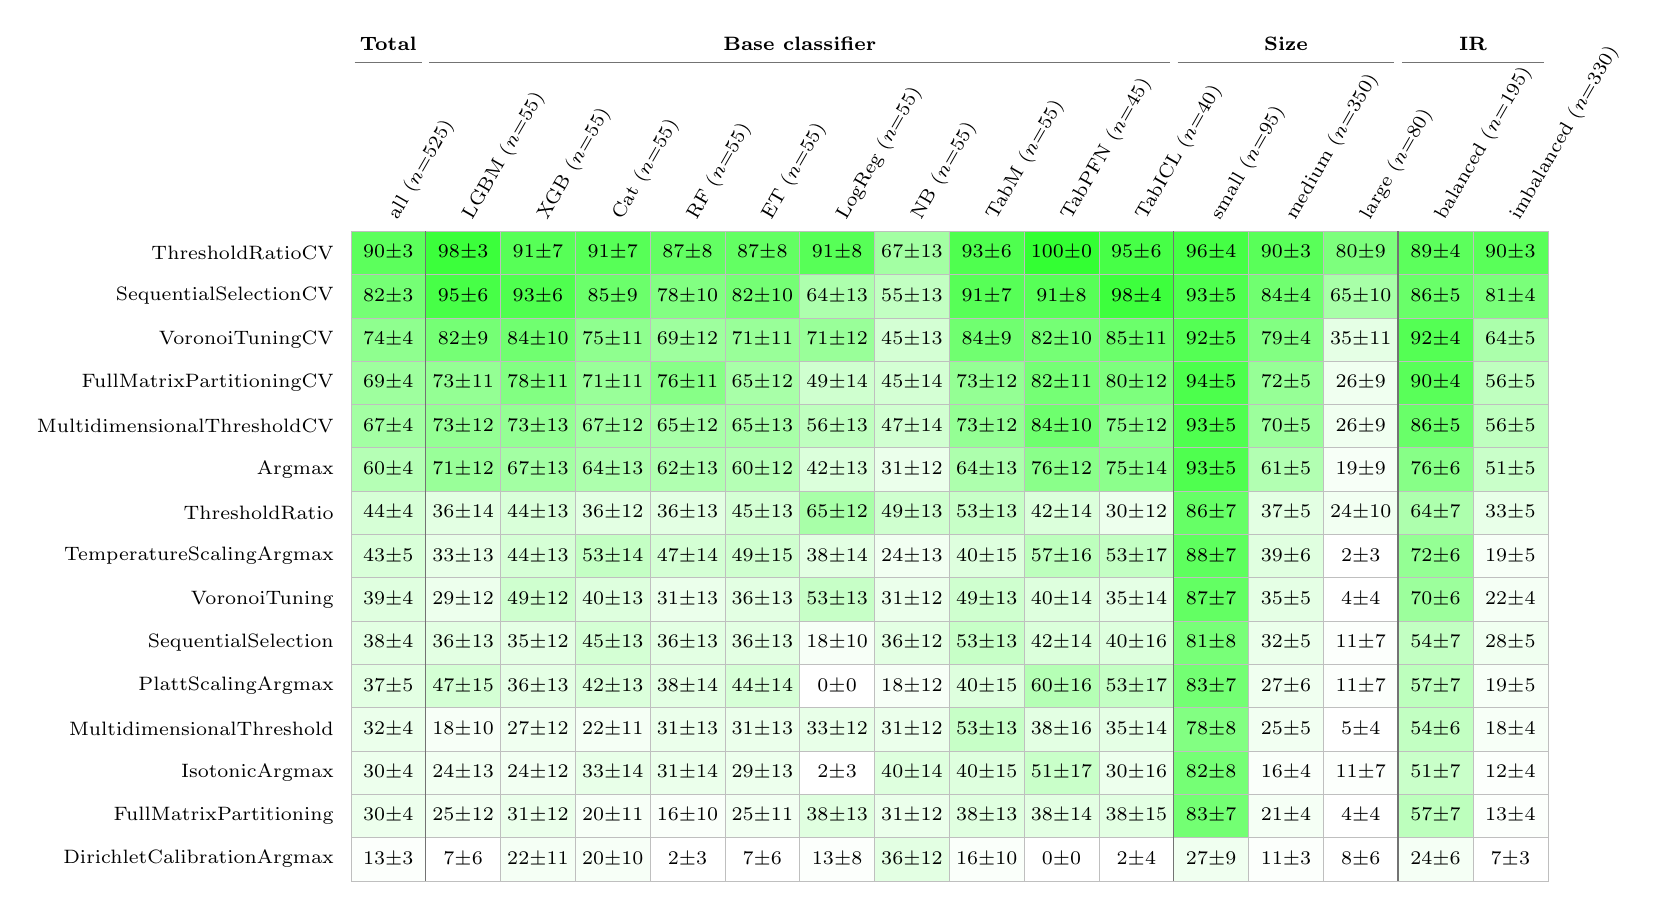
\begin{tikzpicture}[
    x=0.95cm, y=0.55cm,
    cell/.style={rectangle, draw=black!25, line width=0.2pt,
        minimum width=0.95cm, minimum height=0.55cm,
        anchor=center, font=\scriptsize, inner sep=0pt},
    rowlbl/.style={font=\scriptsize, anchor=east},
    collbl/.style={font=\scriptsize, anchor=west, rotate=60},
    grouplbl/.style={font=\scriptsize\bfseries, anchor=south},
    sep/.style={draw=black!55, line width=0.5pt},
]
\node[cell, fill=green!64] at (1, 15) {$90{\pm}3$};
\node[cell, fill=green!77] at (2, 15) {$98{\pm}3$};
\node[cell, fill=green!66] at (3, 15) {$91{\pm}7$};
\node[cell, fill=green!66] at (4, 15) {$91{\pm}7$};
\node[cell, fill=green!61] at (5, 15) {$87{\pm}8$};
\node[cell, fill=green!61] at (6, 15) {$87{\pm}8$};
\node[cell, fill=green!66] at (7, 15) {$91{\pm}8$};
\node[cell, fill=green!36] at (8, 15) {$67{\pm}13$};
\node[cell, fill=green!69] at (9, 15) {$93{\pm}6$};
\node[cell, fill=green!80] at (10, 15) {$100{\pm}0$};
\node[cell, fill=green!72] at (11, 15) {$95{\pm}6$};
\node[cell, fill=green!73] at (12, 15) {$96{\pm}4$};
\node[cell, fill=green!65] at (13, 15) {$90{\pm}3$};
\node[cell, fill=green!51] at (14, 15) {$80{\pm}9$};
\node[cell, fill=green!64] at (15, 15) {$89{\pm}4$};
\node[cell, fill=green!65] at (16, 15) {$90{\pm}3$};
\node[cell, fill=green!54] at (1, 14) {$82{\pm}3$};
\node[cell, fill=green!72] at (2, 14) {$95{\pm}6$};
\node[cell, fill=green!69] at (3, 14) {$93{\pm}6$};
\node[cell, fill=green!58] at (4, 14) {$85{\pm}9$};
\node[cell, fill=green!49] at (5, 14) {$78{\pm}10$};
\node[cell, fill=green!54] at (6, 14) {$82{\pm}10$};
\node[cell, fill=green!32] at (7, 14) {$64{\pm}13$};
\node[cell, fill=green!24] at (8, 14) {$55{\pm}13$};
\node[cell, fill=green!66] at (9, 14) {$91{\pm}7$};
\node[cell, fill=green!66] at (10, 14) {$91{\pm}8$};
\node[cell, fill=green!76] at (11, 14) {$98{\pm}4$};
\node[cell, fill=green!69] at (12, 14) {$93{\pm}5$};
\node[cell, fill=green!56] at (13, 14) {$84{\pm}4$};
\node[cell, fill=green!34] at (14, 14) {$65{\pm}10$};
\node[cell, fill=green!59] at (15, 14) {$86{\pm}5$};
\node[cell, fill=green!52] at (16, 14) {$81{\pm}4$};
\node[cell, fill=green!44] at (1, 13) {$74{\pm}4$};
\node[cell, fill=green!54] at (2, 13) {$82{\pm}9$};
\node[cell, fill=green!56] at (3, 13) {$84{\pm}10$};
\node[cell, fill=green!44] at (4, 13) {$75{\pm}11$};
\node[cell, fill=green!38] at (5, 13) {$69{\pm}12$};
\node[cell, fill=green!40] at (6, 13) {$71{\pm}11$};
\node[cell, fill=green!40] at (7, 13) {$71{\pm}12$};
\node[cell, fill=green!17] at (8, 13) {$45{\pm}13$};
\node[cell, fill=green!56] at (9, 13) {$84{\pm}9$};
\node[cell, fill=green!54] at (10, 13) {$82{\pm}10$};
\node[cell, fill=green!58] at (11, 13) {$85{\pm}11$};
\node[cell, fill=green!67] at (12, 13) {$92{\pm}5$};
\node[cell, fill=green!49] at (13, 13) {$79{\pm}4$};
\node[cell, fill=green!10] at (14, 13) {$35{\pm}11$};
\node[cell, fill=green!67] at (15, 13) {$92{\pm}4$};
\node[cell, fill=green!33] at (16, 13) {$64{\pm}5$};
\node[cell, fill=green!38] at (1, 12) {$69{\pm}4$};
\node[cell, fill=green!42] at (2, 12) {$73{\pm}11$};
\node[cell, fill=green!49] at (3, 12) {$78{\pm}11$};
\node[cell, fill=green!40] at (4, 12) {$71{\pm}11$};
\node[cell, fill=green!47] at (5, 12) {$76{\pm}11$};
\node[cell, fill=green!34] at (6, 12) {$65{\pm}12$};
\node[cell, fill=green!19] at (7, 12) {$49{\pm}14$};
\node[cell, fill=green!17] at (8, 12) {$45{\pm}14$};
\node[cell, fill=green!42] at (9, 12) {$73{\pm}12$};
\node[cell, fill=green!54] at (10, 12) {$82{\pm}11$};
\node[cell, fill=green!51] at (11, 12) {$80{\pm}12$};
\node[cell, fill=green!70] at (12, 12) {$94{\pm}5$};
\node[cell, fill=green!41] at (13, 12) {$72{\pm}5$};
\node[cell, fill=green!6] at (14, 12) {$26{\pm}9$};
\node[cell, fill=green!65] at (15, 12) {$90{\pm}4$};
\node[cell, fill=green!25] at (16, 12) {$56{\pm}5$};
\node[cell, fill=green!36] at (1, 11) {$67{\pm}4$};
\node[cell, fill=green!42] at (2, 11) {$73{\pm}12$};
\node[cell, fill=green!42] at (3, 11) {$73{\pm}13$};
\node[cell, fill=green!36] at (4, 11) {$67{\pm}12$};
\node[cell, fill=green!34] at (5, 11) {$65{\pm}12$};
\node[cell, fill=green!34] at (6, 11) {$65{\pm}13$};
\node[cell, fill=green!25] at (7, 11) {$56{\pm}13$};
\node[cell, fill=green!18] at (8, 11) {$47{\pm}14$};
\node[cell, fill=green!42] at (9, 11) {$73{\pm}12$};
\node[cell, fill=green!57] at (10, 11) {$84{\pm}10$};
\node[cell, fill=green!45] at (11, 11) {$75{\pm}12$};
\node[cell, fill=green!69] at (12, 11) {$93{\pm}5$};
\node[cell, fill=green!39] at (13, 11) {$70{\pm}5$};
\node[cell, fill=green!6] at (14, 11) {$26{\pm}9$};
\node[cell, fill=green!59] at (15, 11) {$86{\pm}5$};
\node[cell, fill=green!25] at (16, 11) {$56{\pm}5$};
\node[cell, fill=green!29] at (1, 10) {$60{\pm}4$};
\node[cell, fill=green!40] at (2, 10) {$71{\pm}12$};
\node[cell, fill=green!36] at (3, 10) {$67{\pm}13$};
\node[cell, fill=green!32] at (4, 10) {$64{\pm}13$};
\node[cell, fill=green!31] at (5, 10) {$62{\pm}13$};
\node[cell, fill=green!29] at (6, 10) {$60{\pm}12$};
\node[cell, fill=green!14] at (7, 10) {$42{\pm}13$};
\node[cell, fill=green!8] at (8, 10) {$31{\pm}12$};
\node[cell, fill=green!32] at (9, 10) {$64{\pm}13$};
\node[cell, fill=green!46] at (10, 10) {$76{\pm}12$};
\node[cell, fill=green!45] at (11, 10) {$75{\pm}14$};
\node[cell, fill=green!69] at (12, 10) {$93{\pm}5$};
\node[cell, fill=green!30] at (13, 10) {$61{\pm}5$};
\node[cell, fill=green!3] at (14, 10) {$19{\pm}9$};
\node[cell, fill=green!47] at (15, 10) {$76{\pm}6$};
\node[cell, fill=green!21] at (16, 10) {$51{\pm}5$};
\node[cell, fill=green!16] at (1, 9) {$44{\pm}4$};
\node[cell, fill=green!11] at (2, 9) {$36{\pm}14$};
\node[cell, fill=green!15] at (3, 9) {$44{\pm}13$};
\node[cell, fill=green!11] at (4, 9) {$36{\pm}12$};
\node[cell, fill=green!11] at (5, 9) {$36{\pm}13$};
\node[cell, fill=green!17] at (6, 9) {$45{\pm}13$};
\node[cell, fill=green!34] at (7, 9) {$65{\pm}12$};
\node[cell, fill=green!19] at (8, 9) {$49{\pm}13$};
\node[cell, fill=green!22] at (9, 9) {$53{\pm}13$};
\node[cell, fill=green!14] at (10, 9) {$42{\pm}14$};
\node[cell, fill=green!7] at (11, 9) {$30{\pm}12$};
\node[cell, fill=green!60] at (12, 9) {$86{\pm}7$};
\node[cell, fill=green!11] at (13, 9) {$37{\pm}5$};
\node[cell, fill=green!5] at (14, 9) {$24{\pm}10$};
\node[cell, fill=green!32] at (15, 9) {$64{\pm}7$};
\node[cell, fill=green!9] at (16, 9) {$33{\pm}5$};
\node[cell, fill=green!15] at (1, 8) {$43{\pm}5$};
\node[cell, fill=green!9] at (2, 8) {$33{\pm}13$};
\node[cell, fill=green!16] at (3, 8) {$44{\pm}13$};
\node[cell, fill=green!23] at (4, 8) {$53{\pm}14$};
\node[cell, fill=green!17] at (5, 8) {$47{\pm}14$};
\node[cell, fill=green!19] at (6, 8) {$49{\pm}15$};
\node[cell, fill=green!11] at (7, 8) {$38{\pm}14$};
\node[cell, fill=green!5] at (8, 8) {$24{\pm}13$};
\node[cell, fill=green!13] at (9, 8) {$40{\pm}15$};
\node[cell, fill=green!26] at (10, 8) {$57{\pm}16$};
\node[cell, fill=green!23] at (11, 8) {$53{\pm}17$};
\node[cell, fill=green!63] at (12, 8) {$88{\pm}7$};
\node[cell, fill=green!12] at (13, 8) {$39{\pm}6$};
\node[cell, fill=green!0] at (14, 8) {$2{\pm}3$};
\node[cell, fill=green!42] at (15, 8) {$72{\pm}6$};
\node[cell, fill=green!3] at (16, 8) {$19{\pm}5$};
\node[cell, fill=green!12] at (1, 7) {$39{\pm}4$};
\node[cell, fill=green!7] at (2, 7) {$29{\pm}12$};
\node[cell, fill=green!19] at (3, 7) {$49{\pm}12$};
\node[cell, fill=green!13] at (4, 7) {$40{\pm}13$};
\node[cell, fill=green!8] at (5, 7) {$31{\pm}13$};
\node[cell, fill=green!11] at (6, 7) {$36{\pm}13$};
\node[cell, fill=green!22] at (7, 7) {$53{\pm}13$};
\node[cell, fill=green!8] at (8, 7) {$31{\pm}12$};
\node[cell, fill=green!19] at (9, 7) {$49{\pm}13$};
\node[cell, fill=green!13] at (10, 7) {$40{\pm}14$};
\node[cell, fill=green!10] at (11, 7) {$35{\pm}14$};
\node[cell, fill=green!61] at (12, 7) {$87{\pm}7$};
\node[cell, fill=green!10] at (13, 7) {$35{\pm}5$};
\node[cell, fill=green!0] at (14, 7) {$4{\pm}4$};
\node[cell, fill=green!39] at (15, 7) {$70{\pm}6$};
\node[cell, fill=green!4] at (16, 7) {$22{\pm}4$};
\node[cell, fill=green!11] at (1, 6) {$38{\pm}4$};
\node[cell, fill=green!11] at (2, 6) {$36{\pm}13$};
\node[cell, fill=green!10] at (3, 6) {$35{\pm}12$};
\node[cell, fill=green!17] at (4, 6) {$45{\pm}13$};
\node[cell, fill=green!11] at (5, 6) {$36{\pm}13$};
\node[cell, fill=green!11] at (6, 6) {$36{\pm}13$};
\node[cell, fill=green!3] at (7, 6) {$18{\pm}10$};
\node[cell, fill=green!11] at (8, 6) {$36{\pm}12$};
\node[cell, fill=green!22] at (9, 6) {$53{\pm}13$};
\node[cell, fill=green!14] at (10, 6) {$42{\pm}14$};
\node[cell, fill=green!13] at (11, 6) {$40{\pm}16$};
\node[cell, fill=green!53] at (12, 6) {$81{\pm}8$};
\node[cell, fill=green!8] at (13, 6) {$32{\pm}5$};
\node[cell, fill=green!1] at (14, 6) {$11{\pm}7$};
\node[cell, fill=green!24] at (15, 6) {$54{\pm}7$};
\node[cell, fill=green!6] at (16, 6) {$28{\pm}5$};
\node[cell, fill=green!11] at (1, 5) {$37{\pm}5$};
\node[cell, fill=green!17] at (2, 5) {$47{\pm}15$};
\node[cell, fill=green!10] at (3, 5) {$36{\pm}13$};
\node[cell, fill=green!14] at (4, 5) {$42{\pm}13$};
\node[cell, fill=green!11] at (5, 5) {$38{\pm}14$};
\node[cell, fill=green!16] at (6, 5) {$44{\pm}14$};
\node[cell, fill=green!0] at (7, 5) {$0{\pm}0$};
\node[cell, fill=green!3] at (8, 5) {$18{\pm}12$};
\node[cell, fill=green!13] at (9, 5) {$40{\pm}15$};
\node[cell, fill=green!29] at (10, 5) {$60{\pm}16$};
\node[cell, fill=green!23] at (11, 5) {$53{\pm}17$};
\node[cell, fill=green!55] at (12, 5) {$83{\pm}7$};
\node[cell, fill=green!6] at (13, 5) {$27{\pm}6$};
\node[cell, fill=green!1] at (14, 5) {$11{\pm}7$};
\node[cell, fill=green!26] at (15, 5) {$57{\pm}7$};
\node[cell, fill=green!3] at (16, 5) {$19{\pm}5$};
\node[cell, fill=green!8] at (1, 4) {$32{\pm}4$};
\node[cell, fill=green!3] at (2, 4) {$18{\pm}10$};
\node[cell, fill=green!6] at (3, 4) {$27{\pm}12$};
\node[cell, fill=green!4] at (4, 4) {$22{\pm}11$};
\node[cell, fill=green!8] at (5, 4) {$31{\pm}13$};
\node[cell, fill=green!8] at (6, 4) {$31{\pm}13$};
\node[cell, fill=green!9] at (7, 4) {$33{\pm}12$};
\node[cell, fill=green!8] at (8, 4) {$31{\pm}12$};
\node[cell, fill=green!22] at (9, 4) {$53{\pm}13$};
\node[cell, fill=green!11] at (10, 4) {$38{\pm}16$};
\node[cell, fill=green!10] at (11, 4) {$35{\pm}14$};
\node[cell, fill=green!49] at (12, 4) {$78{\pm}8$};
\node[cell, fill=green!5] at (13, 4) {$25{\pm}5$};
\node[cell, fill=green!0] at (14, 4) {$5{\pm}4$};
\node[cell, fill=green!24] at (15, 4) {$54{\pm}6$};
\node[cell, fill=green!3] at (16, 4) {$18{\pm}4$};
\node[cell, fill=green!7] at (1, 3) {$30{\pm}4$};
\node[cell, fill=green!5] at (2, 3) {$24{\pm}13$};
\node[cell, fill=green!5] at (3, 3) {$24{\pm}12$};
\node[cell, fill=green!9] at (4, 3) {$33{\pm}14$};
\node[cell, fill=green!8] at (5, 3) {$31{\pm}14$};
\node[cell, fill=green!7] at (6, 3) {$29{\pm}13$};
\node[cell, fill=green!0] at (7, 3) {$2{\pm}3$};
\node[cell, fill=green!13] at (8, 3) {$40{\pm}14$};
\node[cell, fill=green!13] at (9, 3) {$40{\pm}15$};
\node[cell, fill=green!21] at (10, 3) {$51{\pm}17$};
\node[cell, fill=green!7] at (11, 3) {$30{\pm}16$};
\node[cell, fill=green!54] at (12, 3) {$82{\pm}8$};
\node[cell, fill=green!2] at (13, 3) {$16{\pm}4$};
\node[cell, fill=green!1] at (14, 3) {$11{\pm}7$};
\node[cell, fill=green!21] at (15, 3) {$51{\pm}7$};
\node[cell, fill=green!1] at (16, 3) {$12{\pm}4$};
\node[cell, fill=green!7] at (1, 2) {$30{\pm}4$};
\node[cell, fill=green!5] at (2, 2) {$25{\pm}12$};
\node[cell, fill=green!8] at (3, 2) {$31{\pm}12$};
\node[cell, fill=green!3] at (4, 2) {$20{\pm}11$};
\node[cell, fill=green!2] at (5, 2) {$16{\pm}10$};
\node[cell, fill=green!5] at (6, 2) {$25{\pm}11$};
\node[cell, fill=green!12] at (7, 2) {$38{\pm}13$};
\node[cell, fill=green!8] at (8, 2) {$31{\pm}12$};
\node[cell, fill=green!12] at (9, 2) {$38{\pm}13$};
\node[cell, fill=green!11] at (10, 2) {$38{\pm}14$};
\node[cell, fill=green!11] at (11, 2) {$38{\pm}15$};
\node[cell, fill=green!55] at (12, 2) {$83{\pm}7$};
\node[cell, fill=green!4] at (13, 2) {$21{\pm}4$};
\node[cell, fill=green!0] at (14, 2) {$4{\pm}4$};
\node[cell, fill=green!26] at (15, 2) {$57{\pm}7$};
\node[cell, fill=green!1] at (16, 2) {$13{\pm}4$};
\node[cell, fill=green!1] at (1, 1) {$13{\pm}3$};
\node[cell, fill=green!0] at (2, 1) {$7{\pm}6$};
\node[cell, fill=green!4] at (3, 1) {$22{\pm}11$};
\node[cell, fill=green!3] at (4, 1) {$20{\pm}10$};
\node[cell, fill=green!0] at (5, 1) {$2{\pm}3$};
\node[cell, fill=green!0] at (6, 1) {$7{\pm}6$};
\node[cell, fill=green!1] at (7, 1) {$13{\pm}8$};
\node[cell, fill=green!11] at (8, 1) {$36{\pm}12$};
\node[cell, fill=green!2] at (9, 1) {$16{\pm}10$};
\node[cell, fill=green!0] at (10, 1) {$0{\pm}0$};
\node[cell, fill=green!0] at (11, 1) {$2{\pm}4$};
\node[cell, fill=green!6] at (12, 1) {$27{\pm}9$};
\node[cell, fill=green!1] at (13, 1) {$11{\pm}3$};
\node[cell, fill=green!0] at (14, 1) {$8{\pm}6$};
\node[cell, fill=green!4] at (15, 1) {$24{\pm}6$};
\node[cell, fill=green!0] at (16, 1) {$7{\pm}3$};
\node[rowlbl] at (0.4, 15) {ThresholdRatioCV};
\node[rowlbl] at (0.4, 14) {SequentialSelectionCV};
\node[rowlbl] at (0.4, 13) {VoronoiTuningCV};
\node[rowlbl] at (0.4, 12) {FullMatrixPartitioningCV};
\node[rowlbl] at (0.4, 11) {MultidimensionalThresholdCV};
\node[rowlbl] at (0.4, 10) {Argmax};
\node[rowlbl] at (0.4, 9) {ThresholdRatio};
\node[rowlbl] at (0.4, 8) {TemperatureScalingArgmax};
\node[rowlbl] at (0.4, 7) {VoronoiTuning};
\node[rowlbl] at (0.4, 6) {SequentialSelection};
\node[rowlbl] at (0.4, 5) {PlattScalingArgmax};
\node[rowlbl] at (0.4, 4) {MultidimensionalThreshold};
\node[rowlbl] at (0.4, 3) {IsotonicArgmax};
\node[rowlbl] at (0.4, 2) {FullMatrixPartitioning};
\node[rowlbl] at (0.4, 1) {DirichletCalibrationArgmax};
\node[collbl] at (1, 15.6) {all ($n{=}525$)};
\node[collbl] at (2, 15.6) {LGBM ($n{=}55$)};
\node[collbl] at (3, 15.6) {XGB ($n{=}55$)};
\node[collbl] at (4, 15.6) {Cat ($n{=}55$)};
\node[collbl] at (5, 15.6) {RF ($n{=}55$)};
\node[collbl] at (6, 15.6) {ET ($n{=}55$)};
\node[collbl] at (7, 15.6) {LogReg ($n{=}55$)};
\node[collbl] at (8, 15.6) {NB ($n{=}55$)};
\node[collbl] at (9, 15.6) {TabM ($n{=}55$)};
\node[collbl] at (10, 15.6) {TabPFN ($n{=}45$)};
\node[collbl] at (11, 15.6) {TabICL ($n{=}40$)};
\node[collbl] at (12, 15.6) {small ($n{=}95$)};
\node[collbl] at (13, 15.6) {medium ($n{=}350$)};
\node[collbl] at (14, 15.6) {large ($n{=}80$)};
\node[collbl] at (15, 15.6) {balanced ($n{=}195$)};
\node[collbl] at (16, 15.6) {imbalanced ($n{=}330$)};
\draw[black!55, line width=0.5pt] (0.55, 19.4) -- (1.45, 19.4);
\node[grouplbl] at (1.0, 19.45) {Total};
\draw[black!55, line width=0.5pt] (1.55, 19.4) -- (11.45, 19.4);
\node[grouplbl] at (6.5, 19.45) {Base classifier};
\draw[black!55, line width=0.5pt] (11.55, 19.4) -- (14.45, 19.4);
\node[grouplbl] at (13.0, 19.45) {Size};
\draw[black!55, line width=0.5pt] (14.55, 19.4) -- (16.45, 19.4);
\node[grouplbl] at (15.5, 19.45) {IR};
\draw[sep] (1.5, 0.5) -- (1.5, 15.5);
\draw[sep] (11.5, 0.5) -- (11.5, 15.5);
\draw[sep] (14.5, 0.5) -- (14.5, 15.5);
\end{tikzpicture}%
}
\caption{Per-strategy win/tie rates on multiclass maximization metrics. Each cell reads ``$r{\pm}H$'': $r$ is the percentage of (dataset, model, objective) cells in the slice where the strategy won or tied the per-row best under the $\pm 1$ SE overlap rule, and $H$ is the half-width of a 95\% cluster-bootstrap confidence interval for $r$ (percentage points). Shading is a quadratic ($\mathrm{rate}^2$) scale of $r$. Strategies are sorted by overall win rate; ``$n$'' under each column header is the maximum applicable cell count for that slice.}%
\label{fig:win-counts-multiclass-max}
\end{figure}


\section{Summary of multiclass analysis}

The multiclass campaign supports three conclusions.

\begin{enumerate}
    \item The cross-validated tuning variants lead the per-row comparison on both objective groups. On cost objectives three variants share the top within sampling noise: FullMatrixPartitioningCV ($80\%$), RiskPartitioningCV ($79\%$), LinearScalingCV ($78\%$). On maximization metrics ThresholdRatioCV leads at $90\%$.
    \item The calibrate-then-analytical pipelines do not match the leading CV variants on cost (their win-or-tie rates are $30$ to $53\%$). The calibrators are fit on the $10\%$ validation partition while the CV variants use the full $80\%$ pool, so this gap is consistent with a label-budget gap but does not isolate it from other differences.
    \item The richer Voronoi class does not improve on the vector-tuned variants on this benchmark. Counting cells where a Voronoi variant is the unique SE-overlap winning family, the rate is $0.1\%$ on cost cells and $1.2\%$ on maximization cells. This is consistent with the population-level containment of Proposition~\ref{prop:ps_in_vor}: the strict advantage of Theorem~\ref{thm:rotational_dominance} requires a rotational regime the OpenML pool does not appear to concentrate in.
\end{enumerate}
